\documentclass{article}

% Spacing
\usepackage{setspace} \setlength{\parskip}{\baselineskip}% \onehalfspacing{}

% Graphics
\usepackage{graphicx} \graphicspath{ {./images/} }

% Table of Content
\setcounter{tocdepth}{2}

% Code Formatting
\usepackage{minted} \usemintedstyle{pastie}

\newcommand{\js}[1]{\inputminted{javascript}{samples/js/#1.js}}
\def\code#1{\texttt{#1}}

% Positioning
\usepackage{float}

% Colors
\usepackage[dvipsnames]{xcolor}

% Links
\usepackage{hyperref} \hypersetup{ pdftitle={CMSC 124 Final Project},
	pdfstartview={FitH}, colorlinks=true, linkcolor=black, citecolor=black,
	filecolor=black, urlcolor=MidnightBlue, }


\begin{document}

\pagenumbering{gobble}
\begin{titlepage}
	\centering 
\includegraphics[width=1\textwidth]{logo}\par\vspace{1cm}
						 {\scshape\LARGE Documentation \par} \vfill Submitted in Partial
						 Fulfillment of the Requirements\\ in CMSC 129 Software Engineering
						 2 \vfill Miana, Jose Roy C.\\Po, Justin Andre E.\\Sullano, Yul
						 Vincent E.\\Tumulak, Patricia Lexa U.\\Valles, Oscar Vian L.
\end{titlepage}
\newpage
\tableofcontents
\newpage
\pagenumbering{arabic}

\section{Introduction}
\subsection{Problem or Opportunity}
Project manager and developer communication is very important in executing a
project. Good communication between these two enables better estimation of time
and amount of work done. Various communication and project management tools
exist to keep track of the amount of work done --- e.g. Github Projects, Trello,
Scrummate, and Jira. However, these tools do not have an integrated way of
viewing exactly what the current progress of a task is — in the context of
development.

Checking the current commits in a feature branch lets the developers know the
current state of the code base. However, this information is not easily
digestible by the project managers that do not have technical backgrounds.
\subsection{Solution}
Gitrack makes it easier for both. A web application serves as the task board for
the project managers and developers. This contains cards for every feature that
needs to be built. For every commit on a specific feature branch, a resulting
card on a board gets updated. If that feature is now complete, this card will
then be updated accordingly and moved to the correct column.

\section{Technical Documentation}
\subsection{Architectural Diagram}
\begin{figure}[H]
	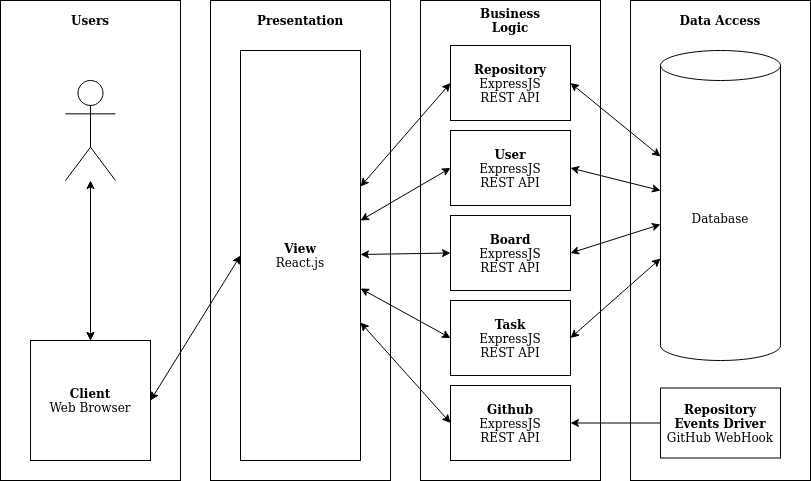
\includegraphics[width=1\textwidth]{arch-diagram}\par\vspace{0.5cm}
	\caption{Architectural Diagram of GiTrack}
	\label{fig:archdiag}
\end{figure}

The architectural style chosen is the layered architecture style. This was
chosen because the application being developed is a web application, and the
nature of most web applications is layered. Gitrack is no different.

This architectural style presents the following advantages: it is modular, it is
maintainable, scalable, and flexible. This allows the team to develop the
application in groups, and allows the application to start small, and expand
later on without much difficulty. Issues and failures can also be easily
addressed and recovered from if only a single layer fails.

The deepest layer is the Data Access layer. This is a database that is powered
by SQLite. This layer stores all of the data for the application. This includes
all of the tasks, repositories, boards, and others. The Repository Events Driver
is a GitHub webhook that sends data to the business logic layer whenever an
event happens on a connected repository

The business logic layer handles sending and receiving data to and from the
Presentation layer using a REST API. This layer also serves and manipulates data
that is stored in the database. This layer will be implemented using ExpressJS

This layer contains the majority of the components of the applications:
repository, users, board, card, and columns. The Repository component handles
connection with the GitHub API, and handles pertinent information like
authentication tokens and branches available. The Users component handles
authentication, and access. This component manages the information about the
user. The Board component manages pertinent data about the board, including the
connected repositories and the columns that the board has. The Column component
manages each column, handling their order and the tasks contained inside. The
Tasks component manages the tasks, this component presents the latest commits,
the assigned developers and project managers, and all other pertinent info. This
component also manages the connected branch and repo to the task.

The presentation layer exposes parts of the program to the users to interact
with. This allows the users to manipulate the cards, add columns, and connect to
the repository. The view portion of the presentation layer will be created using
ReactJS.

\subsection{Frontend}
GiTrack’s frontend was built with \emph{React}, an open-source frontend
JavaScript library for building user interfaces. This library was chosen because
of its flexibility, reusability, reliability, great community support, speed,
and the vast amount of libraries that can be integrated with it. \emph{Redux}
was utilized as the global state container. This is used for storing information
that is to be used throughout the entire application (e.g. user information,
access token, refresh token), minimizing the number of API calls. \emph{Axios},
a promise-based HTTP client, was used to communicate with the backend by
handling the many different HTTP requests that the frontend needs. In order to
properly organize API calls we used a concept known as \emph{services}, wherein
all related endpoints are grouped together and are assigned names to make them
easier to remember.

\begin{figure}[H]
	\js{authservice}
	\caption{Code snippet of AuthService.js}
	\label{fig:authservice}
\end{figure}

\subsection{Backend}
GiTrack’s backend was built using \emph{Express}. Express is a web application
framework that allows for creation of REST APIs with robust routing and high
performance. Important additional dependencies include \emph{bcrypt} and
\emph{jsonwebtoken} for authentication, \emph{@octokit/request} for GitHub API
requests, and \emph{sqlite} and \emph{sqlite3} for communicating with the
database. All of these run on top of \emph{Node.js v15}.

The backend follows the standard REST API standards where different methods,
such as GET, POST, PATCH, PUT, DELETE are used to specify the specific action
that is requested. Information about the specific request can be found in a
couple of different places based on the type of request. GET methods usually
have information pertinent to the request in the URI or as Query parameters. As
an example, the id of the board is placed in the URI when asking for information
about that board: \code{GET /board/{id}}. POST methods have information about
the request in the Request Body.

Schema and documentation for the backend can be found here:
\url{https://api.gitrack.codes/docs/}

\subsection{Database}

\begin{figure}[H]
	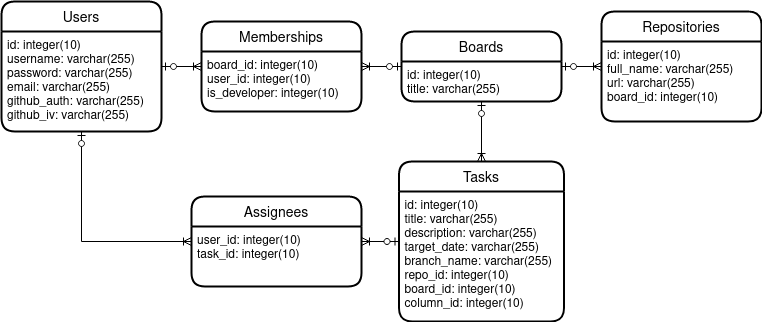
\includegraphics[width=1\textwidth]{erd}\par\vspace{0.5cm}
	\caption{Entity Relationship Diagram}
	\label{fig:erd}
\end{figure}
The GiTrack database uses SQLite and consists of six (6) tables, namely:
\emph{Users}, \emph{Memberships}, \emph{Boards}, \emph{Repositories},
\emph{Tasks}, and \emph{Assignees}. The Entity Relationship Diagram (ERD) in
Figure~\ref{fig:erd} shows the columns in the tables and their corresponding
data types.

The \emph{Users} table lists the users’ data and keys them with an automatically
incremented and unique id. Users’ usernames, passwords, and email addresses are
stored under the \code{username}, \code{password}, and \code{email} columns
respectively. There can only be one account registered to an email address, thus
the values in the \code{email} column must be unique. The same applies for
usernames. The \code{github\_auth} and \code{github\_iv} columns default to
\code{null} on user registration and are only given values when the user
authenticates GiTrack to access their GitHub information. The auth token stored
in \code{github\_auth} is encrypted and the value stored in its respective
\code{github\_iv} column is used to decrypt it.

The \emph{Boards} table lists the project boards in the GiTrack system. The only
columns in this table are the id, which is the primary key, and the board title.
The id of each board is used in other tables to identify the board of which they
are a part.

The \emph{Memberships} table has three columns and no primary key. The columns
are \code{board\_id}, \code{user\_id}, and \code{is\_developer}. The
\code{board\_id} column specifies the board of which the user is a member and
the \code{user\_id} identifies the user based on their unique id. The
\code{is\_developer} column contains flags in the form of 1s and 0s to indicate
whether that user is a developer or a project manager for that board, where a
value of 1 would indicate that the user is a developer and a value of 0 would
indicate that the user is the project manager.

The \emph{Repositories} table lists the repositories used in the GiTrack system.
They are differentiated using the unique \code{id}, which is the primary key. A
repository’s full name, acquired from the GitHub API, is stored under the
\code{full\_name} column. The URL to the repository is stored under the
\code{url} column. Finally, the board to which the repository is assigned is
indicated with the board’s id under the \code{board\_id} column.

The \emph{Tasks} table is the table with the most columns. Columns under this
table are \code{id}, \code{title}, \code{description}, \code{target\_date},
\code{branch\_name}, \code{repo\_id}, \code{board\_id}, and \code{column\_id}.
The \code{id} column serves as the primary key which differentiates task
objects. The \code{title} column contains the title of the tasks and the
\code{description} column contains a more in-depth description of the task to be
done. Task deadlines are stored as strings under the \code{target\_date} column.
The branch where development of the task is specified in \code{branch\_name,}
which is acquired from the GitHub API. The branch has to be a part of the
repository specified by the \code{repo\_id} in the \emph{Repositories} table. In
turn, the repository specified by \code{repo\_id} has to be assigned to the
board specified by the \code{board\_id}, which is the board wherein the task is
assigned. The values in the \code{column\_id} column indicate the status of the
task and is one of three values: 0, 1, or 2. A value of 0 indicates that work
for that task has not been started. A value of 1 indicates that work for that
task is currently ongoing. Finally, a value of 2 indicates that work for that
task has been completed and the task’s branch has been merged to the master
branch of the repository.

Finally, the \emph{Assignees} table has only two columns and no primary key. The
\code{user\_id} column contains the id of the user assigned to the task
specified by the \code{task\_id}. Users can only be assigned to tasks if they
are within the same board.

\subsection{Deployment}
Deployment was done using a single \emph{DigitalOcean} droplet that runs Ubuntu
20.04 (LTS) x64. It has 1 vCPU and a 25GB Disk. \emph{NGINX} was used as a web
server that serves both the frontend and backend. The frontend was served
normally, the backend was served using NGINX as a reverse proxy pointing to
\code{localhost:3000}.

The domain, \code{gitrack.codes} was bought on name.com. The nameservers of the
domain were pointed to the nameservers of DigitalOcean. This was done so that
management of the server and domain all reside on DigitalOcean.

SSL encryption was made possible through Let’s Encrypt and their program
\emph{Certbot}. Three domains were included in the certificate:
\code{gitrack.codes}, \code{www.gitrack.codes}, and \code{api.gitrack.codes}.


\subsection{Signup}
\begin{figure}[H]
	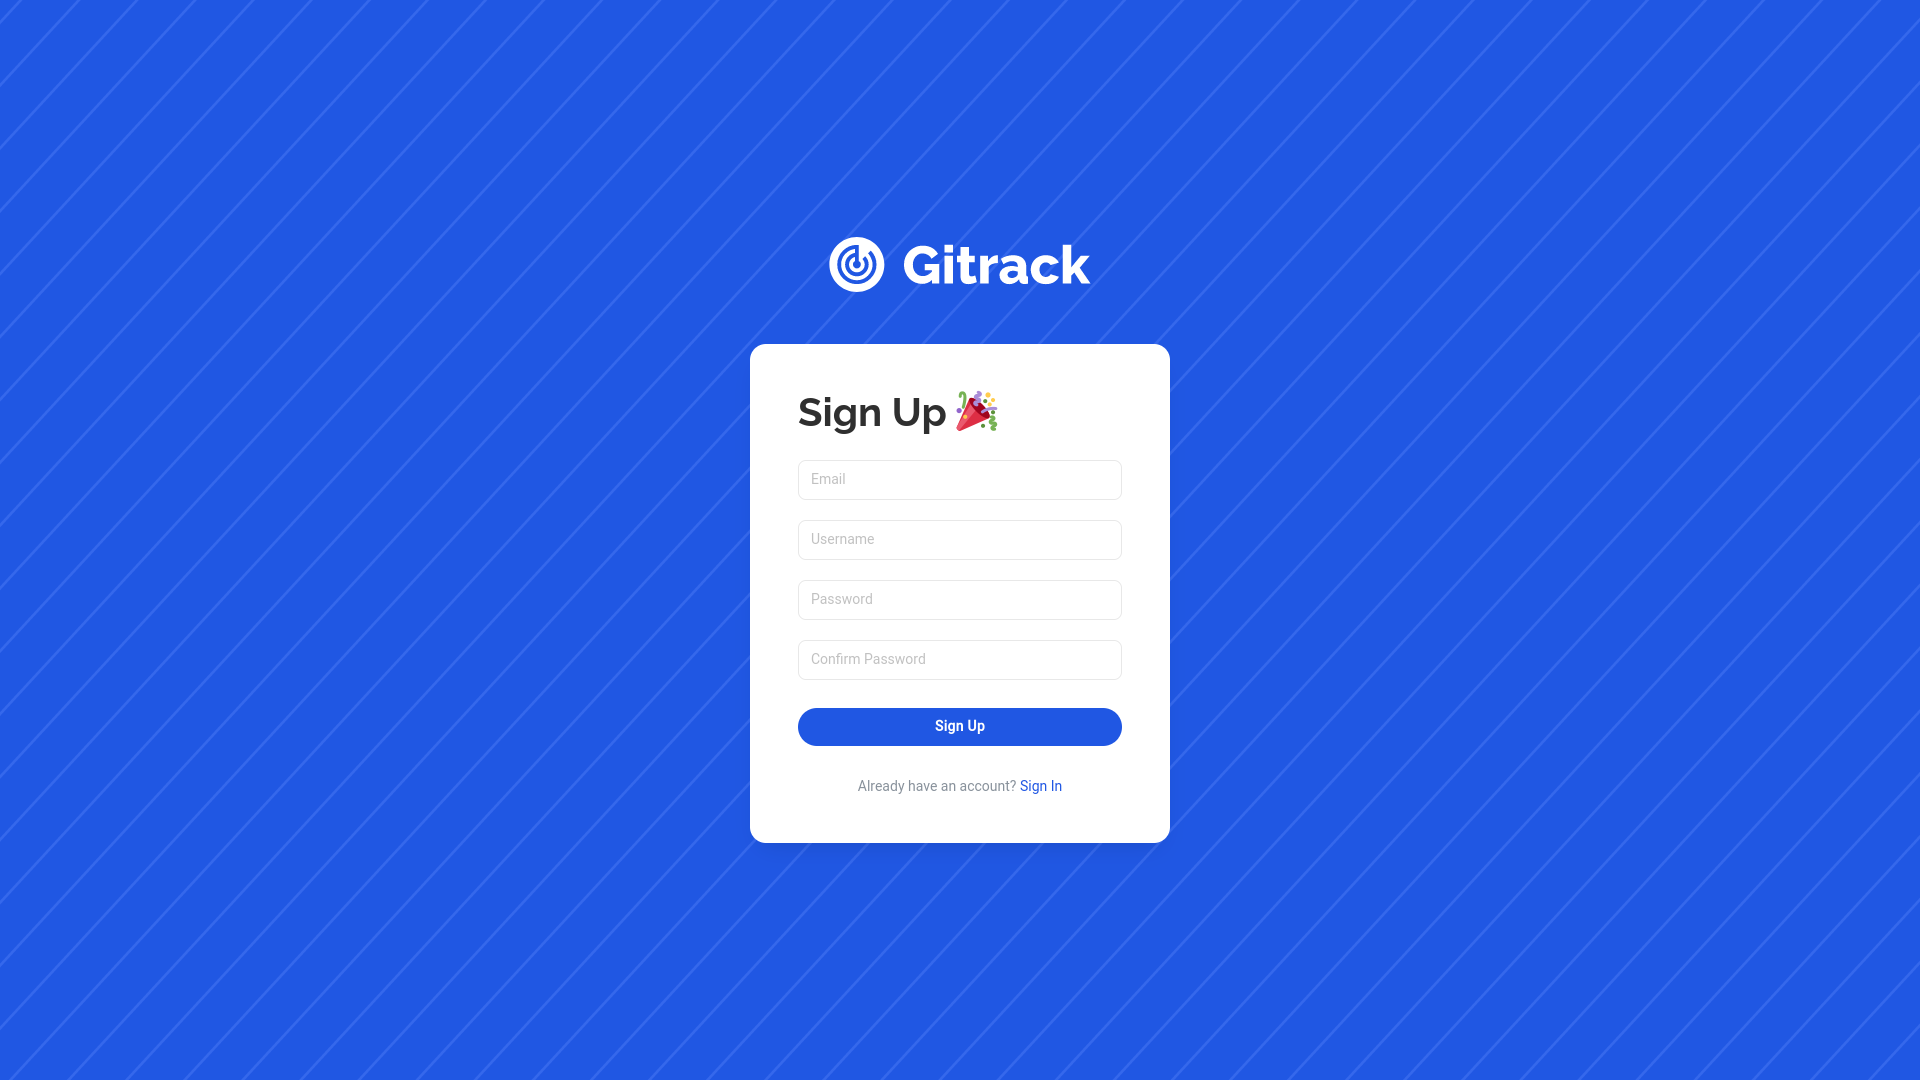
\includegraphics[width=1\textwidth]{signup}\par\vspace{0.5cm}
	\caption{Signup Page}
	\label{fig:signup}
\end{figure}
\subsubsection{Description}
The Signup page, accessed through a link from the Login page, is where one can
create an account for Gitrack. The creation of an account only requires the
user’s email address, their username, and their password. Before submitting
their signup credentials, the user would need to confirm their password.

\subsubsection{Frontend}
The Signup page was built upon a template page called \code{LoginSignup} wherein
the background color and pattern was set. This is also where the routes redirect
between the Login page and the Signup page. This was implemented using the
\code{BrowserRouter} from the \emph{React Router DOM} library.

For the Signup page itself, it’s main components are, as mentioned above, the
template page LoginSignup, the Gitrack logo in white, and a widget called
LoginSignupCard which is used in both the Signup and Login pages. This widget
consists mainly of the title in large text at the top of the card, the input
fields, and the submission button (Sign Up for this page’s case).

Each field requires the corresponding input (Email, Username, Password) in order
to Sign Up. Once the Sign Up button is clicked, it triggers the \code{onSubmit}
function which first checks the inputted passwords. Passwords are hidden during
typing and passwords inputted within the Password and Confirm Password fields
must match. If not, a “Passwords must match” error message appears under the
Confirm Password field. The \code{register()} function from \code{AuthService}
is then called. \code{AuthService} is where the different HTTP requests for each
endpoint needed to login, signup, and logout are written. The \code{register()}
function is a POST request to \code{/auth/register} that sends the email,
username, and password fields as the body. If the server response indicates any
errors such as missing fields, it is caught in a \code{catch} method and an
error message is called indicating the corresponding error. If \code{register()}
was successful, the \code{login()} function is then called with the username and
password as the request body. The global state is then updated with the
information of the user.

\subsubsection{Backend}
This was implemented through a function \code{registerUser()} which accepts the
parameters \code{username}, \code{password}, and \code{email}. The function
encrypts the password using \emph{bcrypt} to keep it secure. If hashing the
password fails, the function throws an error message \code{HASH}, which
indicates there was a problem with hashing. If hashing the password succeeds,
the function will then check if the username already exists within the GiTrack
database. If the username already exists, an error message
\code{DUPLICATE\_USER} will be thrown. If the provided username passes the
existence check, the function will then check if the email exists within the
GiTrack database. If the email is already in use by another user, an error
message \code{DUPLICATE\_EMAIL} will be thrown. When all the checks have
succeeded, the function will try to insert the user information into the Users
table. If, for any reason, inserting the values fails, an error message
\code{INSERT\_FAILED} will be thrown and the error details will be logged in the
console.

The endpoint for this function, \code{/auth/register}, receives a POST request
which contains the user’s \code{username}, \code{password}, and \code{email} in
its request body. The endpoint returns status code 400 if the request body does
not contain values for all of these data, together with error messages
\code{MISSING\_USERNAME}, M\code{ISSING\_PASSWORD}, or \code{MISSING\_EMAIL}. If
the request body is complete, it proceeds to try and register the user with the
given credentials. If either the username or email is already in use, the
endpoint returns status code 409 with the error message \code{DUPLICATE\_EMAIL}
or \code{DUPLICATE\_USER,} depending on which gets thrown first in the
\code{registerUser()} function. If \code{registerUser()} fails for any other
reason, it returns status code 500 with the error message thrown. If
\code{registerUser()} succeeds, the endpoint returns status code 201 and an
empty error message to tell the frontend that registration was successful.

\subsection{Login}
\begin{figure}[H]
	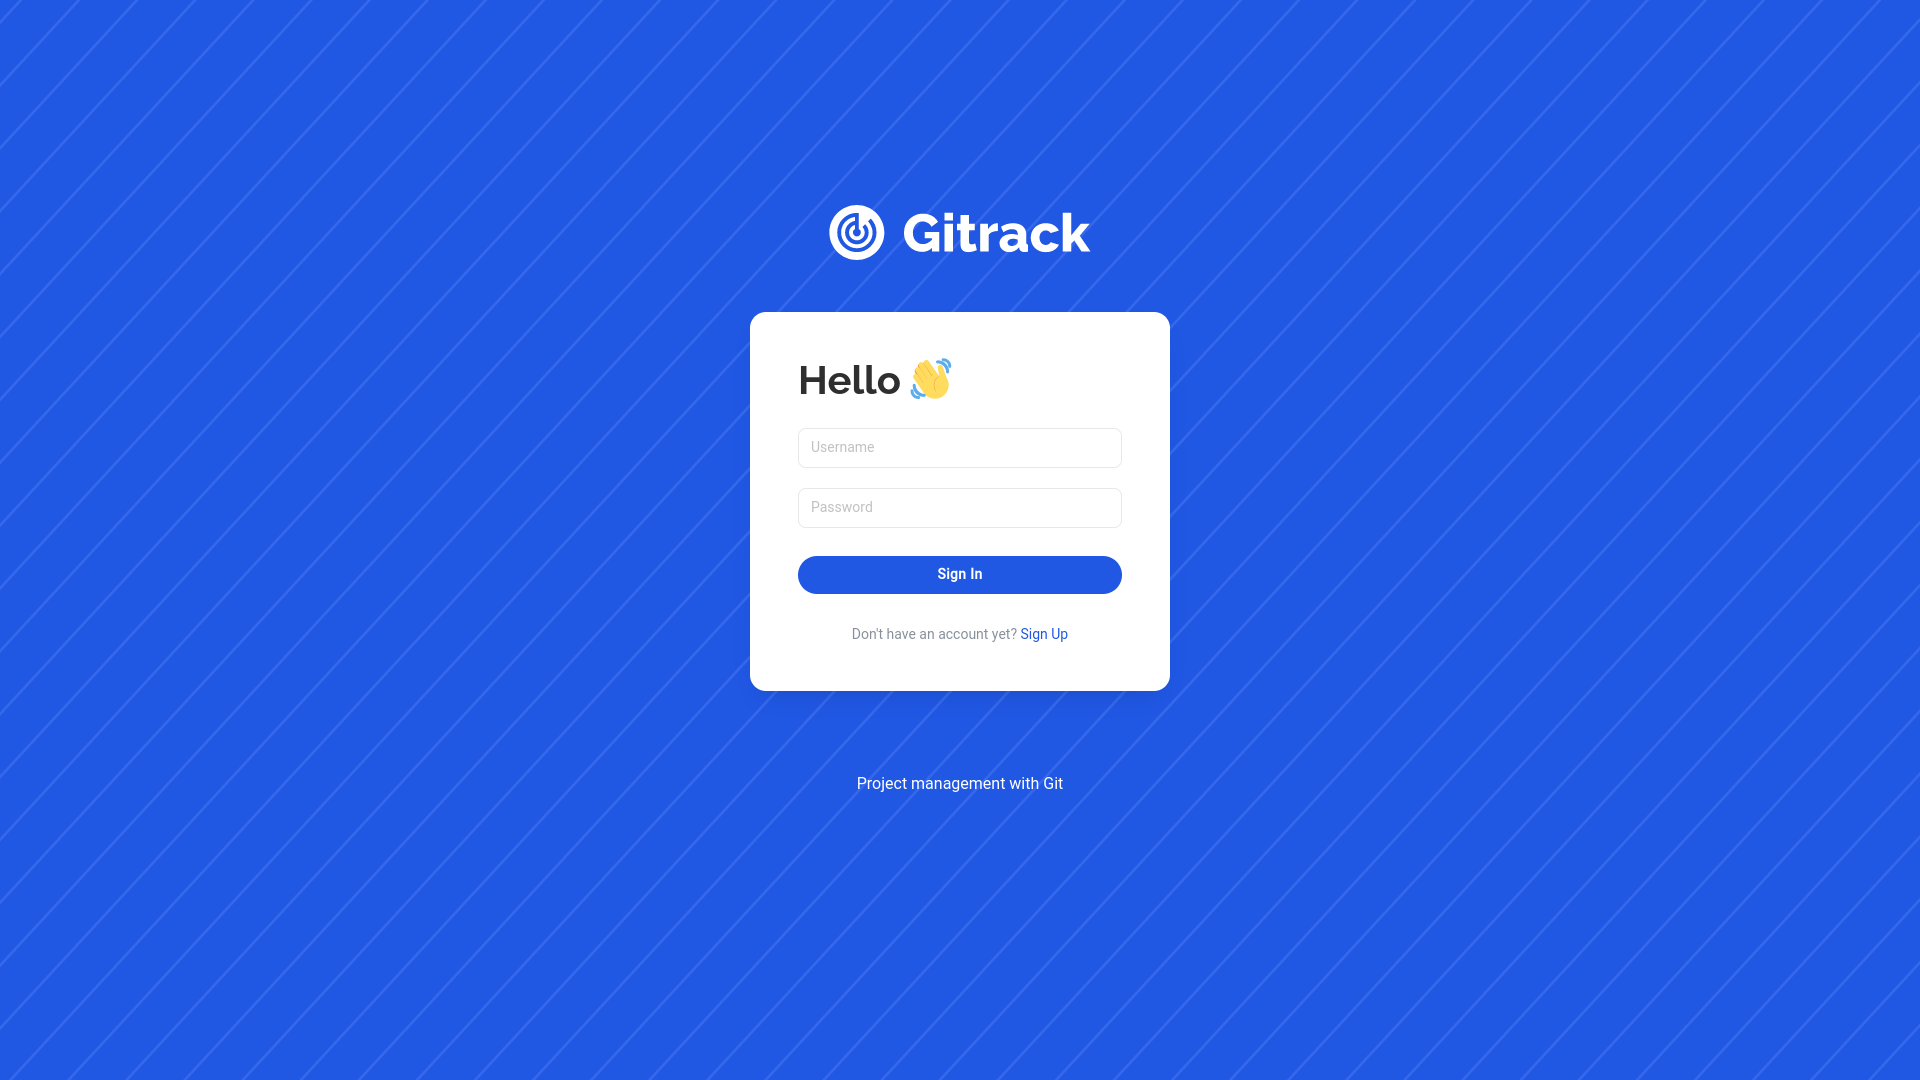
\includegraphics[width=1\textwidth]{login}\par\vspace{0.5cm}
	\caption{Login Page}
	\label{fig:login}
\end{figure}
\subsubsection{Description}
The Login page is the first page that greets the user once they enter the
website. It is how they are able to access the rest of the site by logging in if
they have an existing account or to access the Signup page if they don’t. It
also features a little description of what Gitrack is for --- \emph{``Project
management with Git''.}

\subsubsection{Frontend}
The Login page was built upon the same \code{LoginSignup} page. The only
difference between the Signup and Login pages in terms of the interface are the
title, and number of input fields. The only input required is the Username and
the Password. The submission button is now a “Sign In” button on this page.

If any input fields are missing, an error message is displayed indicating the
missing field required. Once the Sign In button is clicked, an \code{onSubmit()}
function is triggered that first calls the \code{login()} function from
\code{AuthService.} \code{login()} is a POST request to \code{/auth/login} that
sends the username and password as the body. On successful login, the user is
granted access and refresh tokens and the global state is updated. If there are
errors in either the username or password or both, an error message is displayed
indicating “Incorrect username or password.”

A \code{watch()} method is used to listen to any changes made to the username or
password. Errors are cleared if there were any changes made.

\subsubsection{Backend}
This is implemented using the \code{loginUser()} function which accepts the
parameters \code{username} and \code{password}. The function first searches for
the given username in the database. This search will return \code{undefined} if
there is no such \code{username} in the database, and the function will throw an
error message \code{USER\_NOT\_FOUND}. If the search does not return
\code{undefined}, it will return an object with properties \code{username} and
\code{password} with the user’s unique \code{id}, \code{username} and encrypted
\code{password}. The function will then compare the hash of the \code{password}
argument and compare it to the user’s \code{password} in the database. For
security reasons, the function will throw an error message
\code{USER\_NOT\_FOUND} if the password entered by the user does not match the
password in the database after encryption. The function will throw an error
message \code{HASH} if the password check fails for other reasons. Finally, the
function will return the user’s unique \code{id} if all the credentials match.

The endpoint for this, \code{/auth/login}, receives a POST request which
contains the user’s \code{username}, \code{password}, and \code{email} in its
request body and returns a JSON with the properties \code{id}, \code{username},
\code{access\_token}, \code{refresh\_token}, and \code{error\_message}. If
either of these values are missing, the endpoint returns status code 400 with
error message \code{MISSING\_PASSWORD} or \code{MISSING\_USERNAME}. If both of
these are present, the system will try to log the user into the system using the
\code{id} returned from the \code{loginUser()} function. This id will then be
used to sign a JSON Web Token (JWT) and grant the user an access token and a
refresh token. The refresh token is added to the list of refresh tokens for
every user who has logged in, which will be checked if the user would request
for a new access token, and deleted upon logging out. If \code{loginUser()}
throws the \code{USER\_NOT\_FOUND} error message, meaning the entered password
does not match the password in the database, the endpoint returns a status code
403 with the JSON containing null values for all properties except the
\code{error\_message} property, which will be \code{USER\_NOT\_FOUND}. If either
the access token or refresh token signing fails, the endpoint returns a status
code 500 with a JSON similar to the one returned with code 403, with an
\code{error\_message} corresponding to the error thrown by JWT. If no operation
fails, the endpoint returns a status code 200 with a JSON containing the
\code{id} of the user, the user’s \code{username}, their \code{access\_token},
their \code{refresh\_token}, and an \code{error\_message} of null.


\subsection{Main Dashboard}
\begin{figure}[H]
	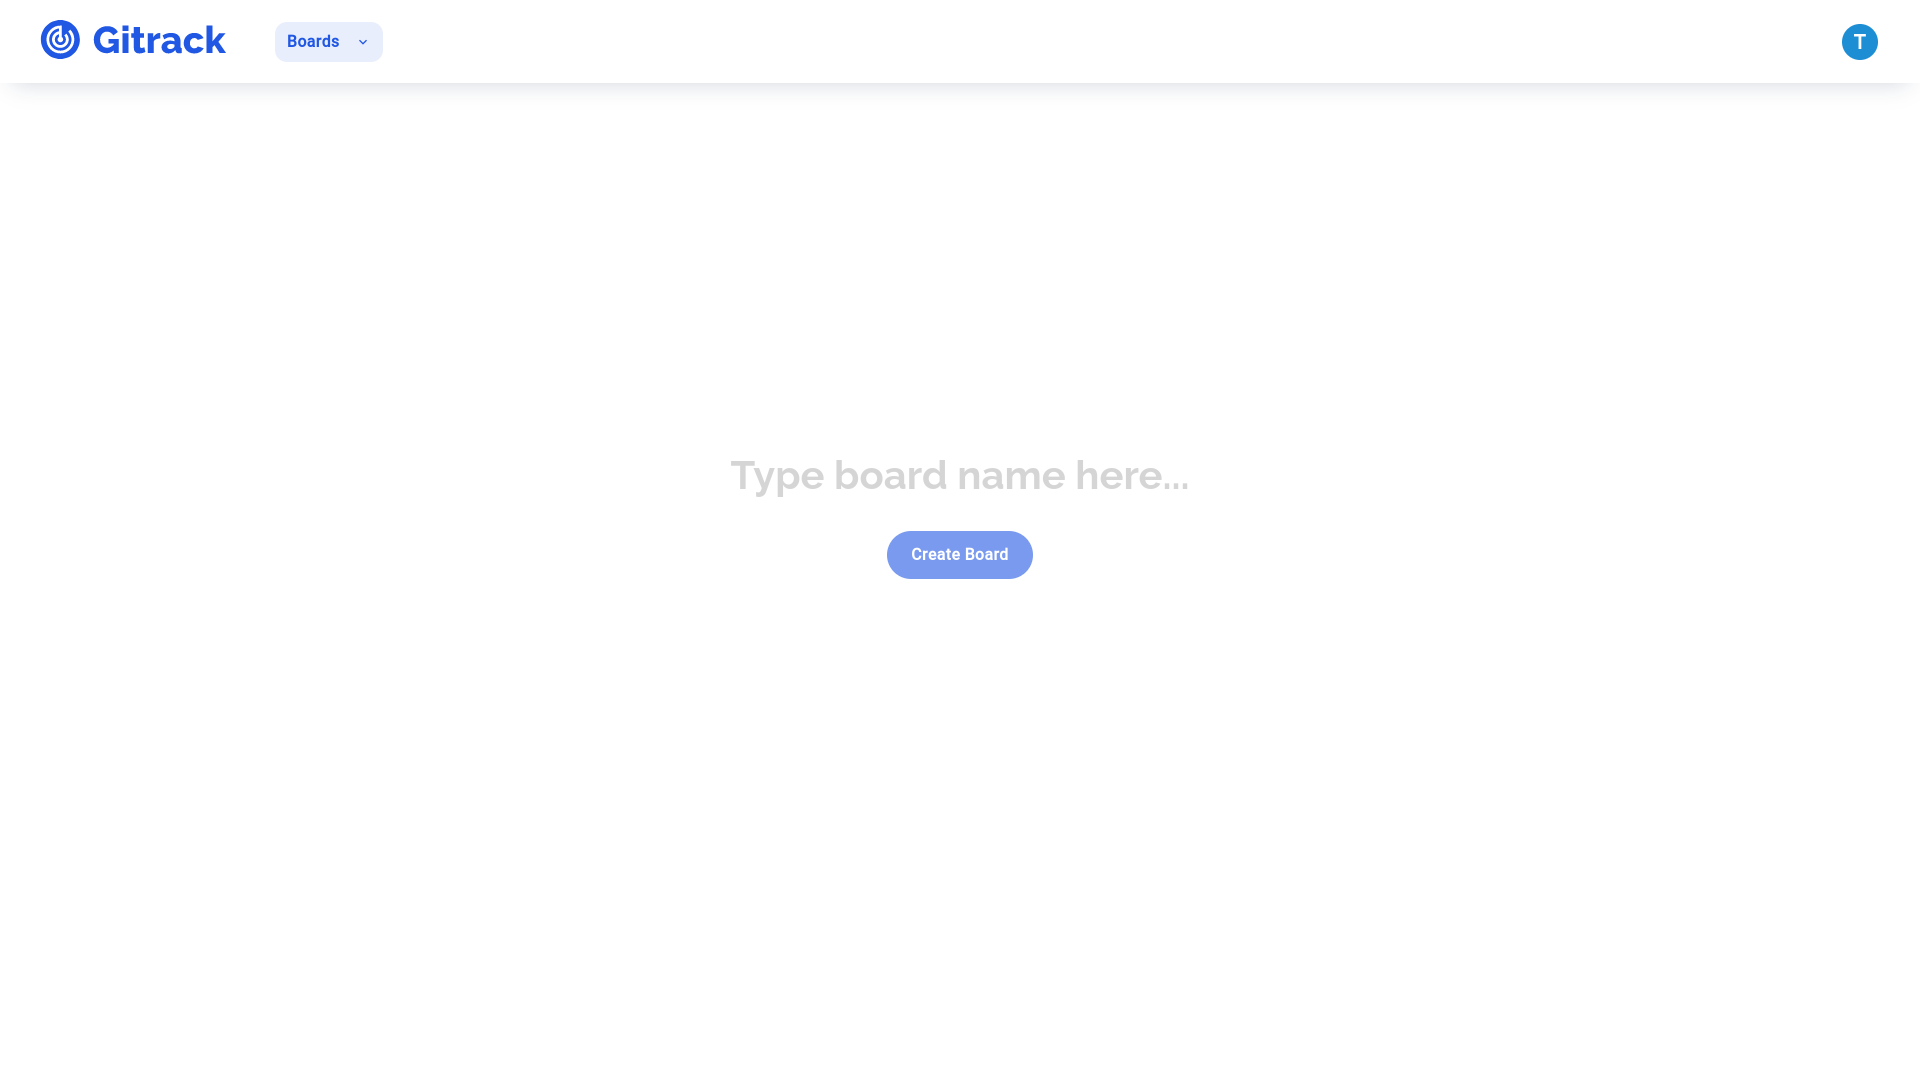
\includegraphics[width=1\textwidth]{create-board}\par\vspace{0.5cm}
	\caption{Create Board}
	\label{fig:create-board}
\end{figure}

\begin{figure}[H]
	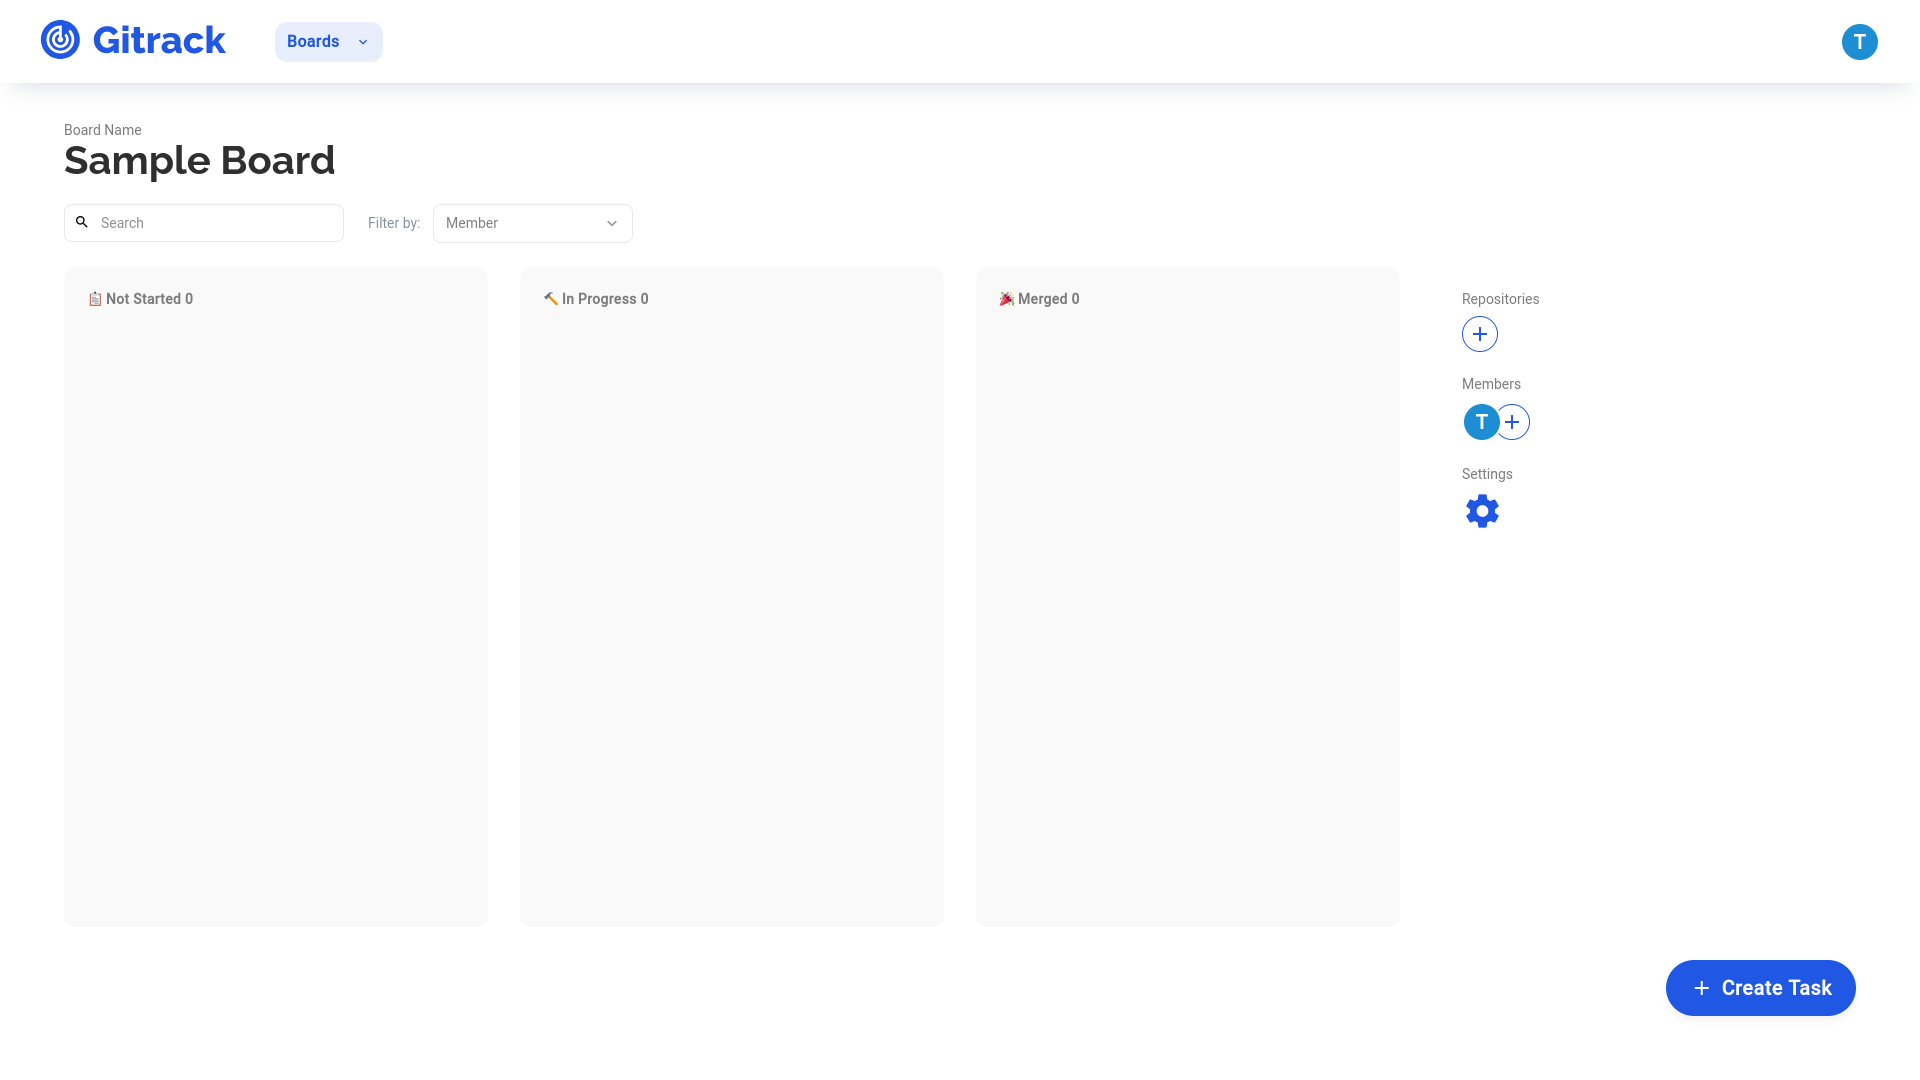
\includegraphics[width=1\textwidth]{board}\par\vspace{0.5cm}
	\caption{Main Dashboard}
	\label{fig:board}
\end{figure}

\begin{figure}[H]
	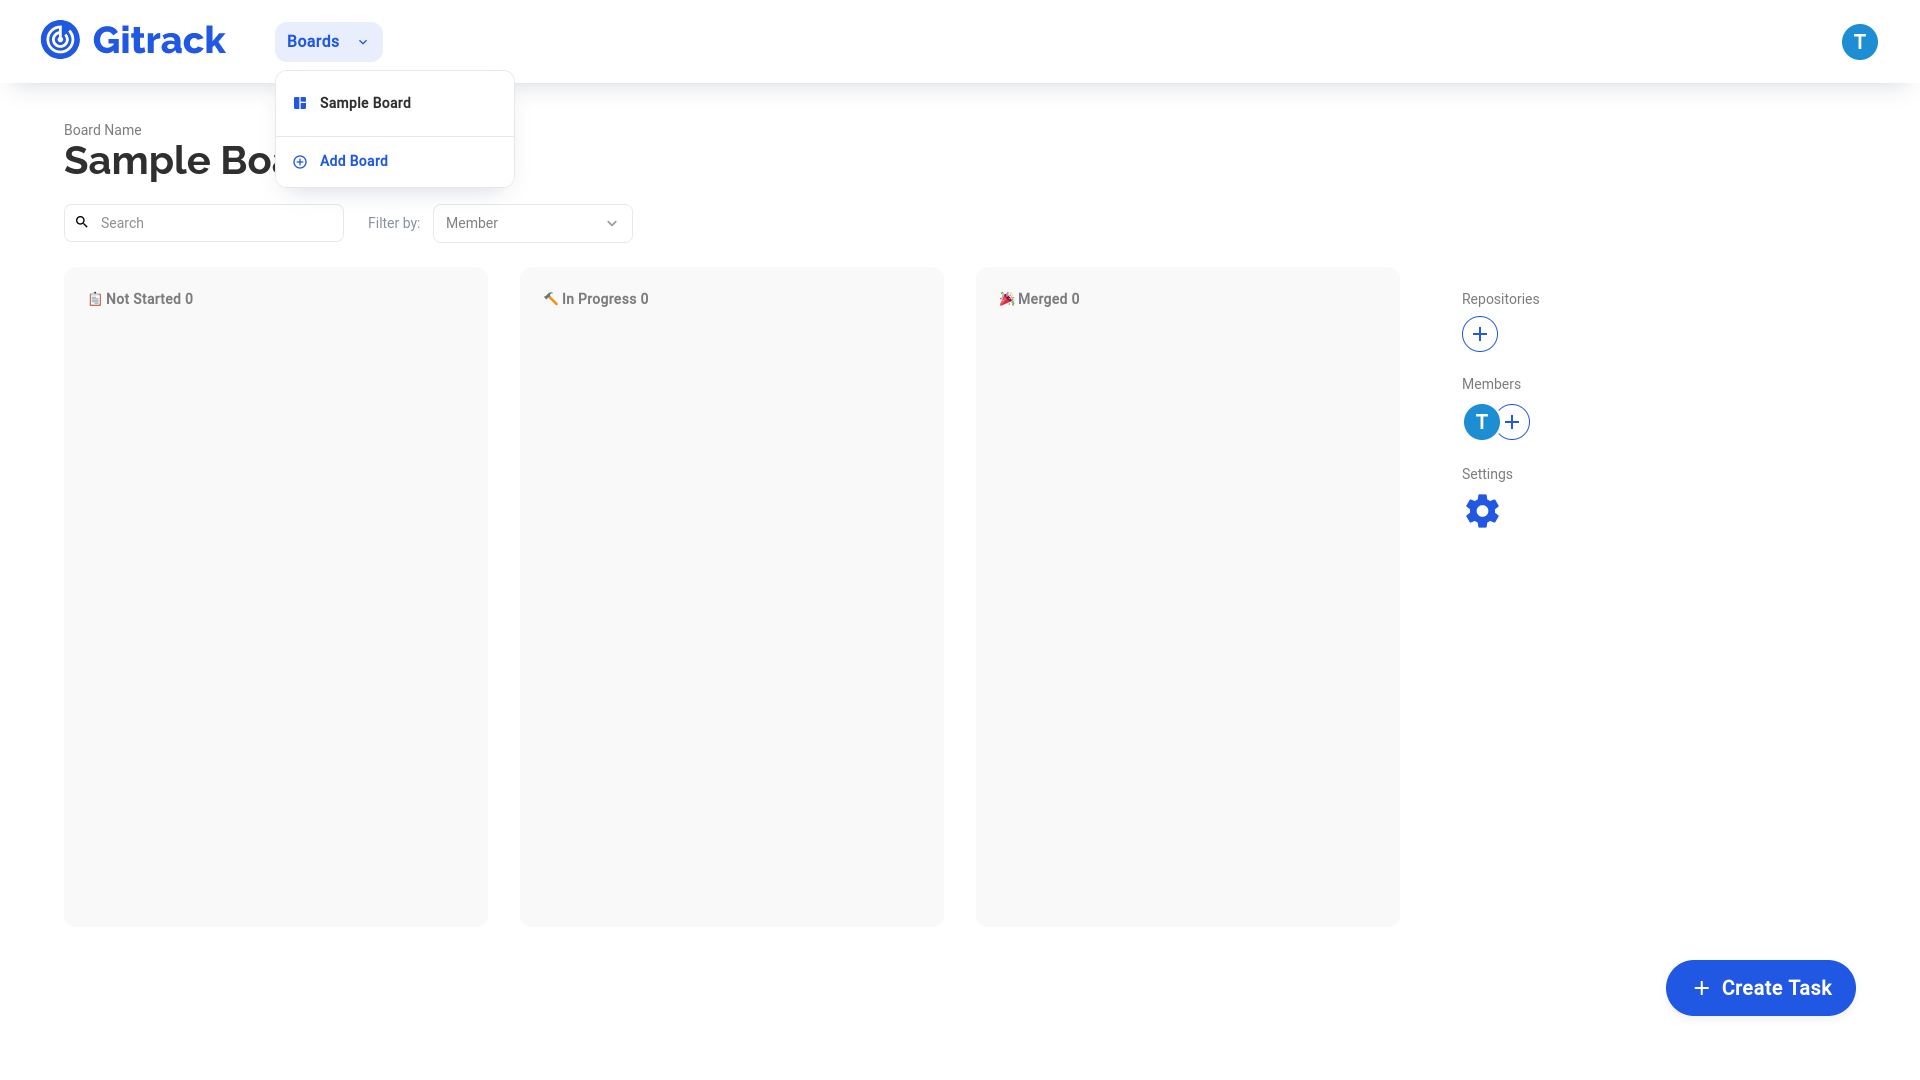
\includegraphics[width=1\textwidth]{board-dropdown}\par\vspace{0.5cm}
	\caption{Boards Dropdown}
	\label{fig:board-dropdown}
\end{figure}

\begin{figure}[H]
	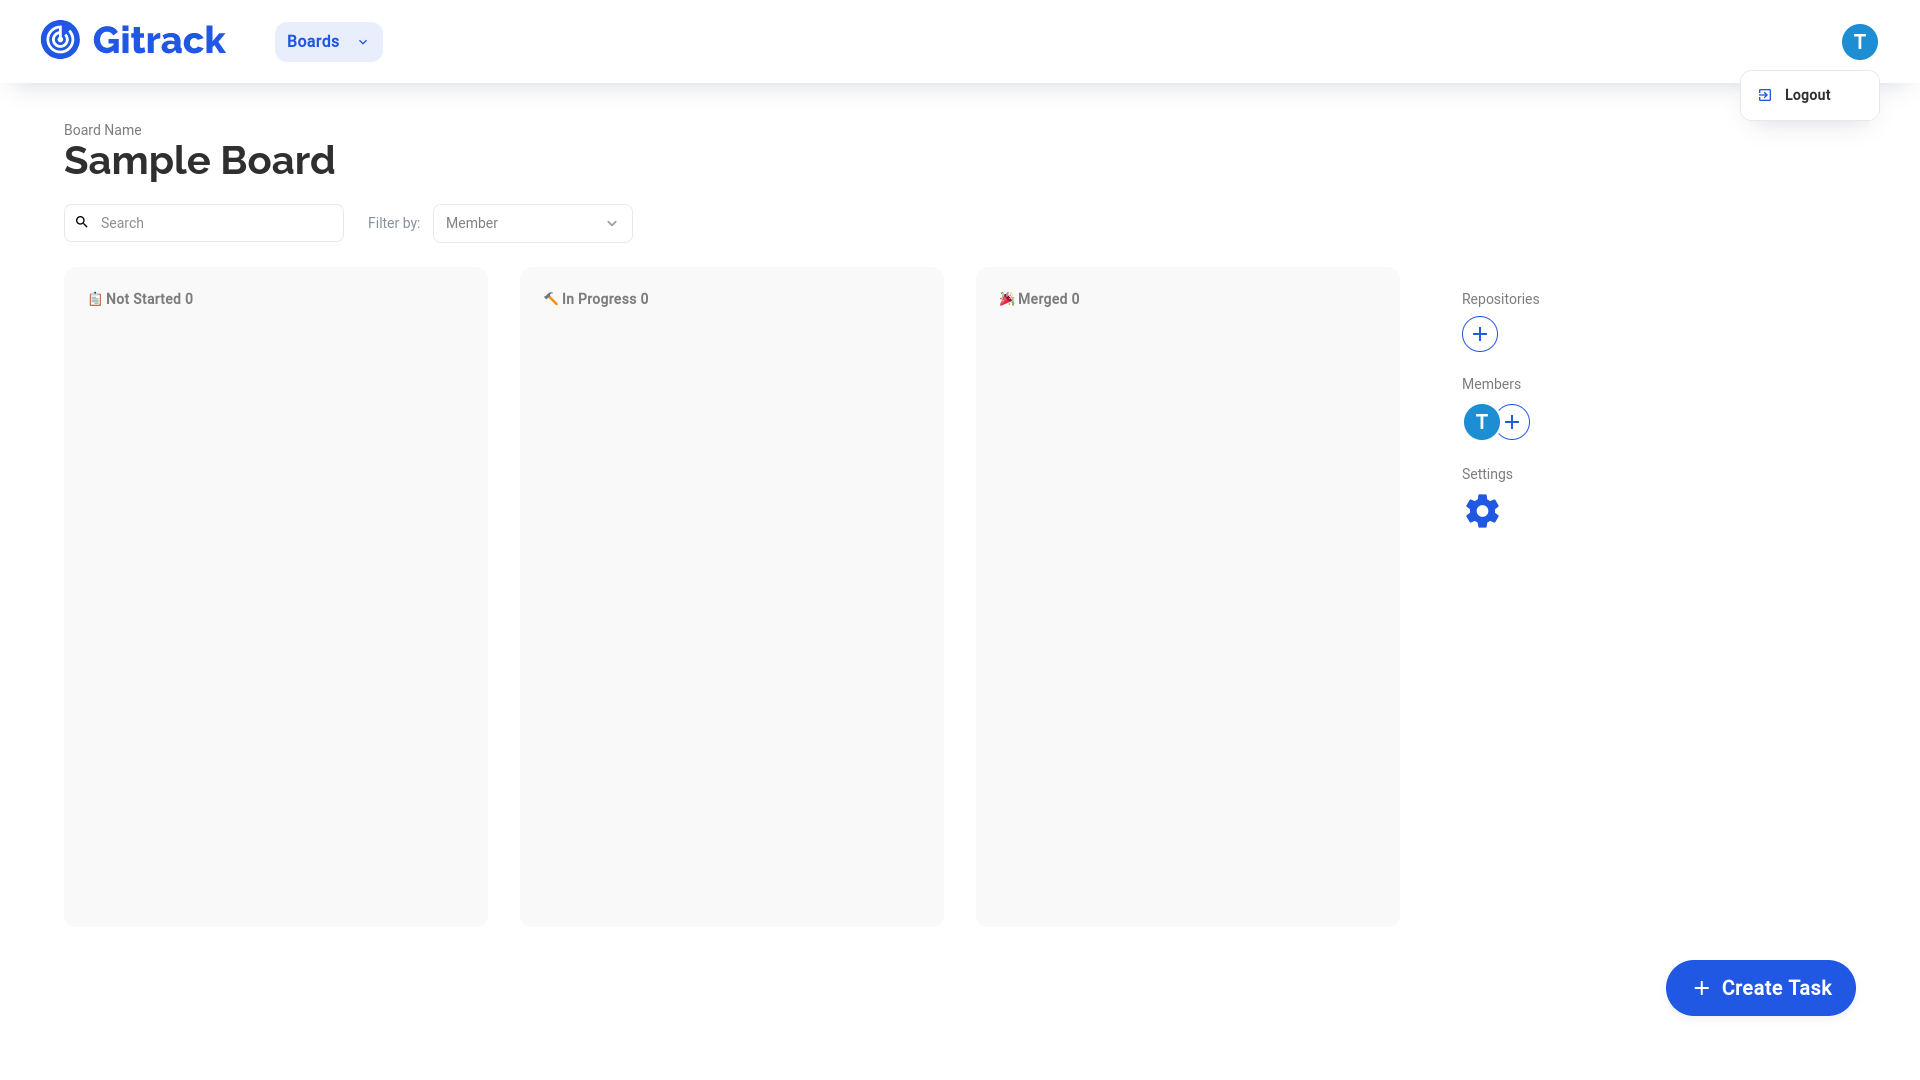
\includegraphics[width=1\textwidth]{board-user}\par\vspace{0.5cm}
	\caption{User Dropdown}
	\label{fig:board-user}
\end{figure}

\begin{figure}[H]
	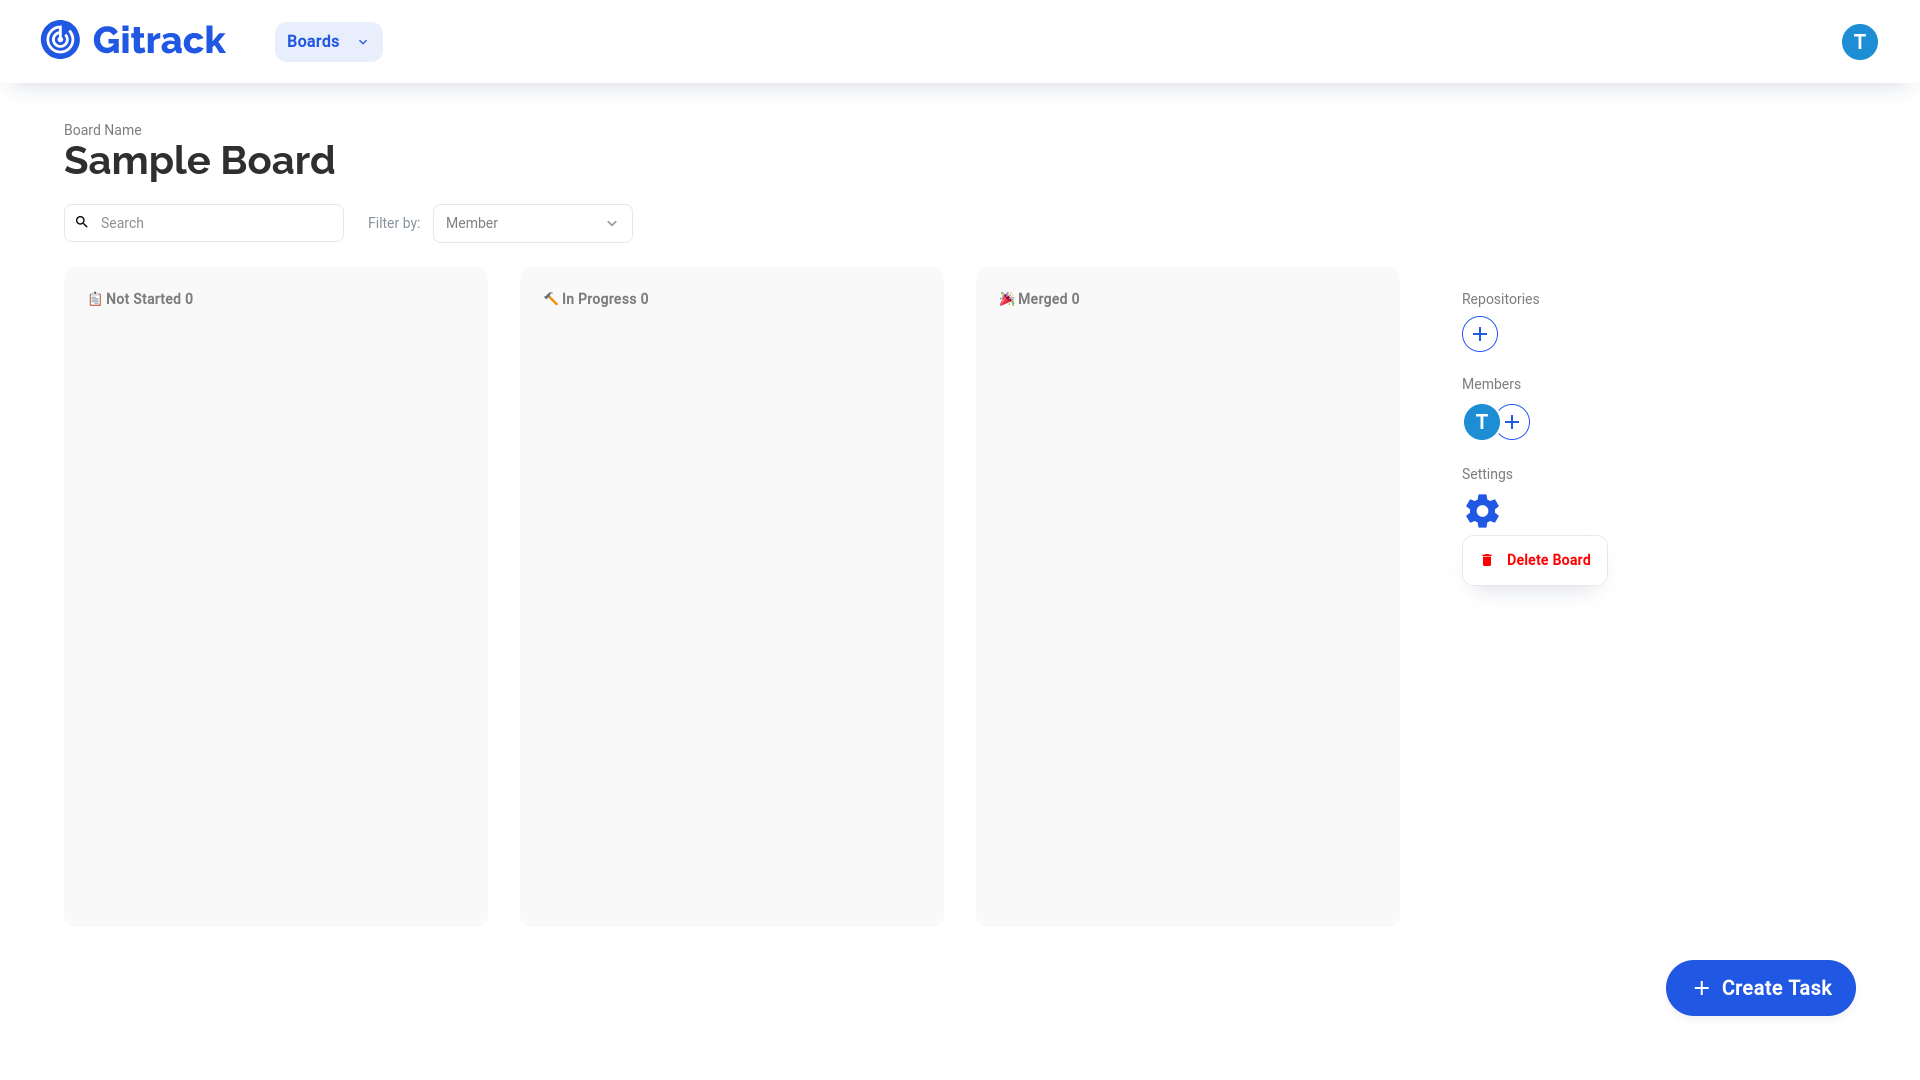
\includegraphics[width=1\textwidth]{board-delete}\par\vspace{0.5cm}
	\caption{Delete Board}
	\label{fig:board-delete}
\end{figure}

\subsubsection{Description}
The Main Dashboard is the core component of the application. This gives the user
access to five main features: creating a new board, viewing information related
to the board (e.g. tasks, repositories, and members), navigating to other
boards, logging out of their account, and deleting the board they are currently
on.

\subsubsection{Frontend}
The Main Dashboard is wrapped in a parent route known as board, which handles
the navigation of routes that share the same UI elements as the dashboard. This
makes sure that the navigation bar is rendered in all of the screens that
require it. Create Board

Once the user has finished signing up, they will immediately be redirected to
the Create Board screen. They are simply presented with an input for the board
name and a button to create it. When the “Create” button is clicked it will
trigger an \code{onClick()} function that would call the \code{create()}
function from the \code{BoardService}. \code{create()} is a POST request to
\code{/board} that receives the board’s name as its body. If successful, it
would then call the \code{refreshBoards()} function which would retrieve the new
list of boards for the Boards Dropdown and redirect them to the url of the new
board.

\paragraph{Dashboard}
When the user is redirected to the new board, the \code{retrieveTasks()},
\code{retrieveRepos()}, and \code{retrieveMembers()} functions from the
\code{BoardService} are simultaneously called once the component is mounted. All
three functions are GET requests that retrieve the information needed for the
board. If a repository has already been linked to the board then the branches
endpoint from \code{GithubService} is then called to retrieve the different
branches of the linked repositories. Once all of the necessary information has
been retrieved, the frontend would then display the user interface that contains
the board’s name, its members, its repositories, and its tasks, which are
wrapped in three different columns representing the progress of each task. The
user could also search for specific tasks and even filter tasks by assignee
using the input and dropdown above the columns respectively.

\paragraph{Navigation Bar}
The navigation bar at the top of the screen contains two components that allow
the user to navigate their way through the application. First is the Boards
Dropdown, which contains the list of boards that the user is currently on, as
well as the ability to add a new board. Clicking on any of the boards would
redirect the user to the selected board. The second one, the User Dropdown,
allows the user to simply log out of their account when necessary by clicking
the “Logout” button. Clicking the button would trigger a call to the \code{logout()}
function from the \code{AuthService}.

\paragraph{Delete Board}
Finally, the Main Dashboard component also allows the user to delete the board
they are currently on. Once the user clicks the gear icon, it would display a
dropdown that includes the option to delete the board. If clicked, a modal would
be displayed asking for confirmation, and once confirmed, would call the
\code{remove()} function of \code{BoardService} and refresh the list of boards in the Boards
Dropdown.

\subsubsection{Backend}
\paragraph{Create Board}
This component was implemented through \code{createBoard()} function which
accepts the parameters \code{title}, and \code{userId}. To create the board, the
title is inserted into the \emph{Boards} table. The user is also inserted into
the \emph{Memberships} table along with the board it corresponds to, and it's
\code{is\_developer} is set 0 which means that the user is not a developer. If
successful, it then returns the last ID of the \emph{Boards} table. Otherwise,
throws an error message of \code{INSERT\_FAILED}.

For its endpoint, \code{boards/}, receives a POST request where it accepts title
from the request body, and \code{id} from the user. It also returns a JSON with
keys \code{id}, \code{title}, and \code{error\_message}. It first checks if the
title is \code{undefined.} If it is, then it responds with 400 status code,
returns \code{null} value for the JSON keys, and an error of
\code{MISSING\_TITLE} for the \code{error\_message} key. If the title is
defined, it then tries and calls \code{createBoard()} function. If the board was
created or inserted into the database successfully, it returns a JSON with
\code{boardId} for the id key, \code{title} key, and a null
\code{error\_message} key. If unsuccessful, it responds with 500 status code,
returns a JSON with null value on its keys, and the error thrown by the
\code{createBoard()} for the \code{error\_message} key.

\paragraph{Delete Board}
This was implemented using the \code{deleteBoard()} function which accepts the
URI parameter \code{id}, which specifies the id of the board to be deleted from
the database. This function deletes all data related to the board specified by
\code{id} across all tables. \code{deleteBoard()} does this by making five
sequential delete queries to the database in order to delete all rows where
\code{board\_id} equals \code{id}. It first deletes all repositories linked to
the board from the \emph{Repositories} table. It then deletes all assignments in
the \emph{Assignees} table where the assigned tasks in the \emph{Tasks} table
are part of the board. Following this, all tasks in the \emph{Tasks} table which
belong to the board are deleted. It then removes all the users in the
\emph{Memberships} table if they are part of the pard. Finally, it deletes the
board from the \emph{Boards} table. If any of these queries fail,
\code{deleteBoard()} throws an error message \code{DELETE\_FAILED}.

This endpoint, \code{boards/:id(\textbackslash}{\textbackslash{}d+)}, receives a
DELETE request where the request parameter is the \code{id} of the board to be
deleted. This endpoint returns an object that contains the \code{id} of the
board, the board’s \code{title,} and an \code{error\_message}. It also makes use
of \code{userId}, the unique id of the user. If the \code{id} request parameter
is missing, the endpoint returns a status code 400 and an object with null
values for the \code{id} and \code{title} and an \code{error\_message} of
\code{MISSING\_ID}. It then checks if the current user has permission to perform
this delete operation using the \code{getPermissions()} function, which checks
if the current user is a developer or a project manager. If the user does not
have permissions, the endpoint returns a status code 403 with an object with
null values for the id and title and the \code{error\_message} thrown by
\code{getPermissions()}. The endpoint then checks if the board exists using
\code{getBoardById()} and stores its returned board object in variable
\code{board}. the board variable receives an object with properties \code{id}
and \code{title}. The endpoint then tries to perform \code{deleteBoard()}. If
\code{deleteBoard()} fails, it returns status code 500 and an object with
\code{null} values for the \code{id} and \code{title} and the
\code{error\_message} thrown by \code{deleteBoard()}. If \code{deleteBoard()}
succeeds, it returns status code 200 and an object with the value of the
\code{id} property of the object stored in board, the value of the \code{title}
property of the object stored in board, and an \code{error\_message} of \code{null}.

\paragraph{Get All Tasks In Board}
This functionality was implemented by the function \code{getTaskinBoard().} This
function has one argument, \code{boardId}. This argument is used to get all
tasks in the \emph{Task} table that has its \code{board\_id} set to
\code{boardId.} Once all tasks has been retrieved, all assignees of the tasks
are then queried from the \emph{Assignees} table. Once all assignees have been
found, these information is then returned. If for some reason these queries have
failed, an error, \emph{TASK\_NOT\_FOUND} is thrown.

The endpoint of this is located at
\code{/boards/:id(\textbackslash{}\textbackslash{}d+)/tasks} and is requested
with a GET method. This endpoint has \code{id} as a request parameter and uses
\code{userId} from the request user. If \code{id} is missing, the endpoint
immediately returns a status code of 400, nulls other keys and sets
\code{error\_message} to be \code{MISSING\_ID}. If \code{id} is present,
permissions of the user are checked using \code{getPermissions()}. If
permissions are not enough the endpoint returns a status code 403 with an object
with null values for \code{tasks} and the \code{error\_message} thrown by
\code{getPermissions()}. If permissions are enough, \code{getTasksInBoard()} is
called with \code{id} as an argument. The endpoint then returns \code{tasks} and
\code{null} for the \code{error\_message.} If there were errors during querying
the tasks, a status code of 500 is returned and the pertinent error code is sent
in \code{error\_message}.

\paragraph{Get All Members In Board}
\code{getMembersInBoard()} is used to implement this functionality. This
function has \code{boardId} as its parameter. This function gets the \code{id} and
\code{username} of all users found in the \emph{Memberships} table that has their \code{board\_id} set
to \code{boardId}. If there were issues querying this information, \code{GET\_FAILED} is
thrown.

The endpoint to access this data is
\code{/boards/:id(\textbackslash{}\textbackslash{}d+)/members}. This endpoint
checks if \code{id} is defined in the request parameters. If it is not, the
endpoint immediately returns a status code of 400, nulls all keys in the return
body, and sets \code{error\_message} to be \code{MISSING\_ID}. If it passes this
check, the \code{id} is then validated to determine if \code{id} points to an
actual board. If not, a status code of 400 is returned, all of the keys in the
return body are set to null, and \code{error\_message} is set to
\code{NOT\_FOUND}. After all those checks were passed by the request,
\code{getMembersInBoard()} is called. The return body has \code{board\_id} set
to \code{id}, \code{members} set to the return value of
\code{getMembersInBoard()}, and \code{error\_message} is set to \code{null}.

\paragraph{Get Repositories Connected to the Board}
\code{getRepositoriesInBoard()} returns all repositories that are connected to a
board. This function receives \code{boardId} as an argument. A query is then
done on the \emph{Repositories} table to get all rows where \code{board\_id} is
set to \code{boardId}. These rows are then returned.

\code{/boards/:id(\textbackslash{}\textbackslash{}d+)/repos} is the endpoint
that calls this function. This endpoint has \code{id} as a request parameter,
and uses \code{userId} stored in the request user. First, \code{id} is checked
to make sure that it is set. If it is not, then a status code is set to 400, all
keys in the response body are set to null and \code{error\_message} is set to
\code{MISSING\_ID}. Afterwards permissions are checked using
\code{getPermissions()} as usual. If permissions are not enough the endpoint
returns a status code 403 with an object with null values for \code{members} and
the \code{error\_message} thrown by \code{getPermissions().} If it passes both
checks, \code{getRepositoriesInBoard()} is called with id as the argument. The
return value of this is then set as repos in the return body.
\code{error\_message} is also set as \code{null.} If any other errors occur, the
endpoint returns a status code of 500 and \code{error\_message} is set to the
error message.

\paragraph{Get Branches of all Repositories}
Two distinct functions make this functionality possible: \code{getGithubToken()}
and \code{getRepository()}. \code{getGithubToken()} has one parameter,
\code{id}. \code{id} is used to get \code{github\_auth} and \code{github\_iv} of
the user from the database. If no authentication was found, an error,
\code{NOT\_GITHUB\_AUTHENTICATED}, is thrown. Otherwise, the GitHub token is
decrypted using the iv and the token. \code{getRepository()} has one parameter,
\code{id}. This \code{id} is used to get the \code{full\_name} of the repository
from the \emph{Repositories} database.

To get the branches of a repository, a GET request is sent to
\code{/github/:id(\textbackslash{}\textbackslash{}d+)/branches}. This endpoint
requires \code{id} as a request parameter and \code{userId} from the request
user. If \code{id} is not set, the endpoint returns a status code of 400 and a
return body with all keys set to null except \code{error\_message} which is set
to \code{MISSING\_REPO\_ID}. After checking if all needed data is present, the
GitHub oauth token is requested using \code{getGithubToken()}. Afterwards, the
full name of the repository is obtained using \code{getRepository()}. After
these two information are available, a GET request is then sent to
\code{/repos/{owner}/{repo}/branches} using \code{@octokit/request} to get the
branches of a repository. These branches are then returned and
\code{error\_message} is set to \code{null}. If an error occurs from the
request, a 403 status code is returned, all keys are set to null in the request
body, and \code{error\_message} is set to \code{NOT\_GITHUB\_AUTHENTICATED}. If
any other error occurs, a 500 status codes is sent and the \code{error\_message}
is set to the error message of the error.

\subsection{Github Authentication}
\begin{figure}[H]
	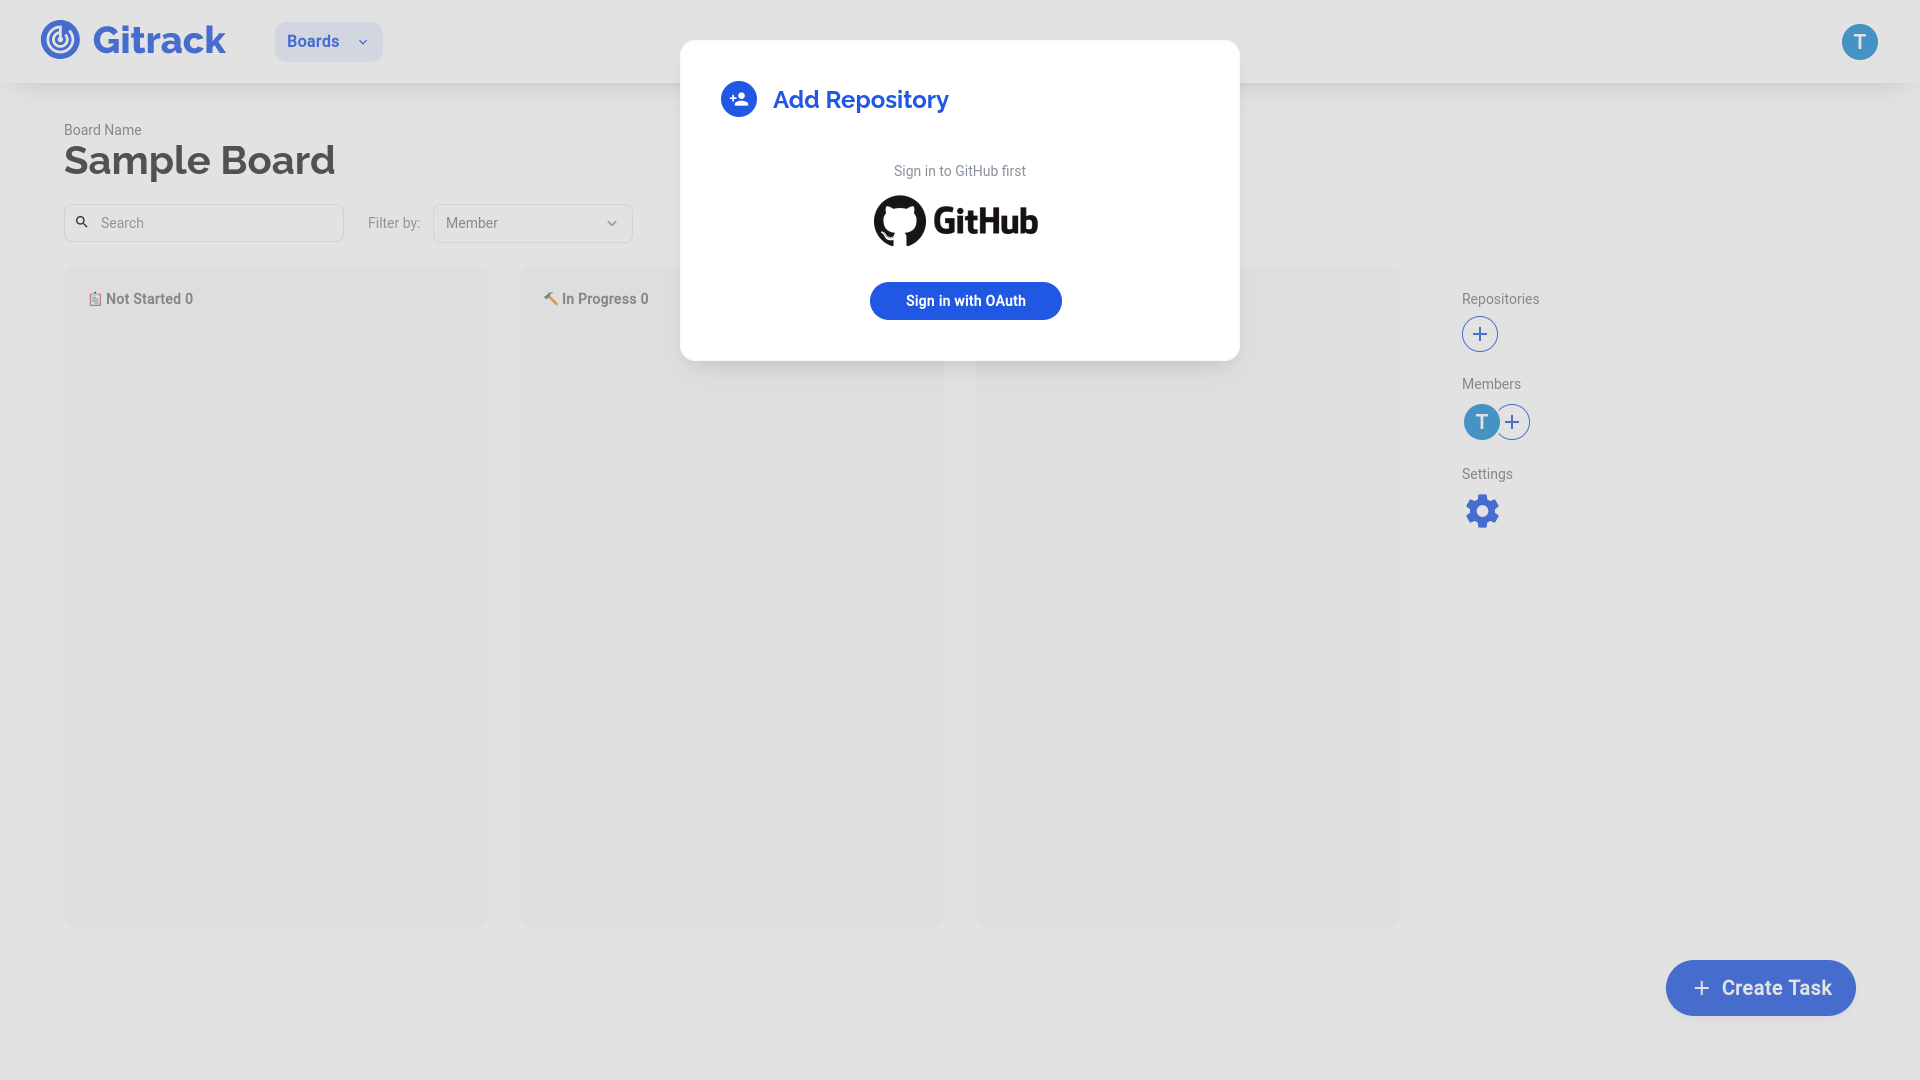
\includegraphics[width=1\textwidth]{github-auth}\par\vspace{0.5cm}
	\caption{Github Authentication Modal}
	\label{fig:github-auth}
\end{figure}
\subsubsection{Description}
Authenticating with GitHub is a core part of the application. This allows for
connecting a board to a repository, and a task to a specific branch. Other core
functionality of the application builds upon these two features.

\subsubsection{Frontend}
Clicking on the button to add a repository while a user has not connected their
GitHub account will bring up the Github Authentication Modal which is defined by
the \code{SigninGithubModal} component. This component calls the \code{link()}
function under \code{GitHubService}. This function is a GET request to
\code{/github/link} which returns a link for the user to access in order to
allow authorization on GitHub. Once authorized, GitHub redirects the user to
\code{https://gitrack.codes/github/} with \code{code} and \code{state} as query
parameters. These parameters are used for the \code{callback()} function in
\code{GithubService}. This function is a GET request to
\code{/github/link/callback}. If the request was successful, the user is
redirected to the boards page. Otherwise, the user is asked to retry the
authentication process once again. All of the interactions in the URI are
implemented by the \code{Github} component.

\subsubsection{Backend}
This functionality is handled through two endpoints: \code{/github/link},
\code{/github/link/callback}. \code{/github/link} generates a custom URI for
users to click on. This link is a link for
\code{https://github.com/login/oauth/authorize}. This link has additional
parameters added: \code{scope}, \code{client\_id}, and \code{state}.
\code{scope} is the permissions that the application requests from the user. For
GiTrack, this is the permission to modify repositories and to write webhooks.
\code{client\_id} is the Client ID for the OAuth application that was generated
in GitHub. \code{state} is a randomly generated string that is used to validate
the request for authorization. This is checked by both GitHub and by the
application in succeeding requests.

After the user has allowed GiTrack these permissions, The frontend sends a
request to \code{/link/callback} with two parameters: \code{code}, and
\code{state}. These two queries come from GitHub and are used to continue the
authentication flow. State is the exact same state that was created in
\code{/github/link}. If the \code{state} received does not match a \code{state}
stored in memory, this callback is rejected. If the \code{state} was present,
these two parameters are used to send a POST request to
\code{https://github.com/login/oauth/access\_token} which receives the following
data in its request body: \code{code}, \code{state}, \code{client\_id}, and
\code{client\_secret}. \code{code} and \code{state} are the two parameters,
\code{client\_id} is the ID for the OAuth application and \code{client\_secret}
is a secret generated by GitHub to verify if the client is really the client and
not a third party attacker. This endpoint returns an access token that is to be
used for all privileged requests to GitHub in the future. This includes private
repositories, writing webhooks, and others.

This access token is stored in the database using the function
\code{addGithubToken()}. This function has two arguments: \code{id}, and
\code{githubAuthToken}. \code{id} is the ID of the user and
\code{githubAuthToken} is the auth token. This function encrypts the token using
\emph{AES-192-CTR}. The encryption returns two values, a token and the
initialization vector. These two values are stored in the database under the
columns \code{github\_auth} and \code{github\_iv} respectively. The auth token
is encrypted because this allows a lot of permissions for anyone that has access
to this token. If it falls into the wrong hands, this may destroy the entire
GitHub account of the user

If the user already is authenticated, \code{addGithubToken()} throws an error
message: \code{ALREADY\_GITHUB\_AUTHENTICATED}. The endpoint returns a 500
status code with the error message. Otherwise, it simply returns a 200 status
code.

\subsection{Add Repository}
\begin{figure}[H]
	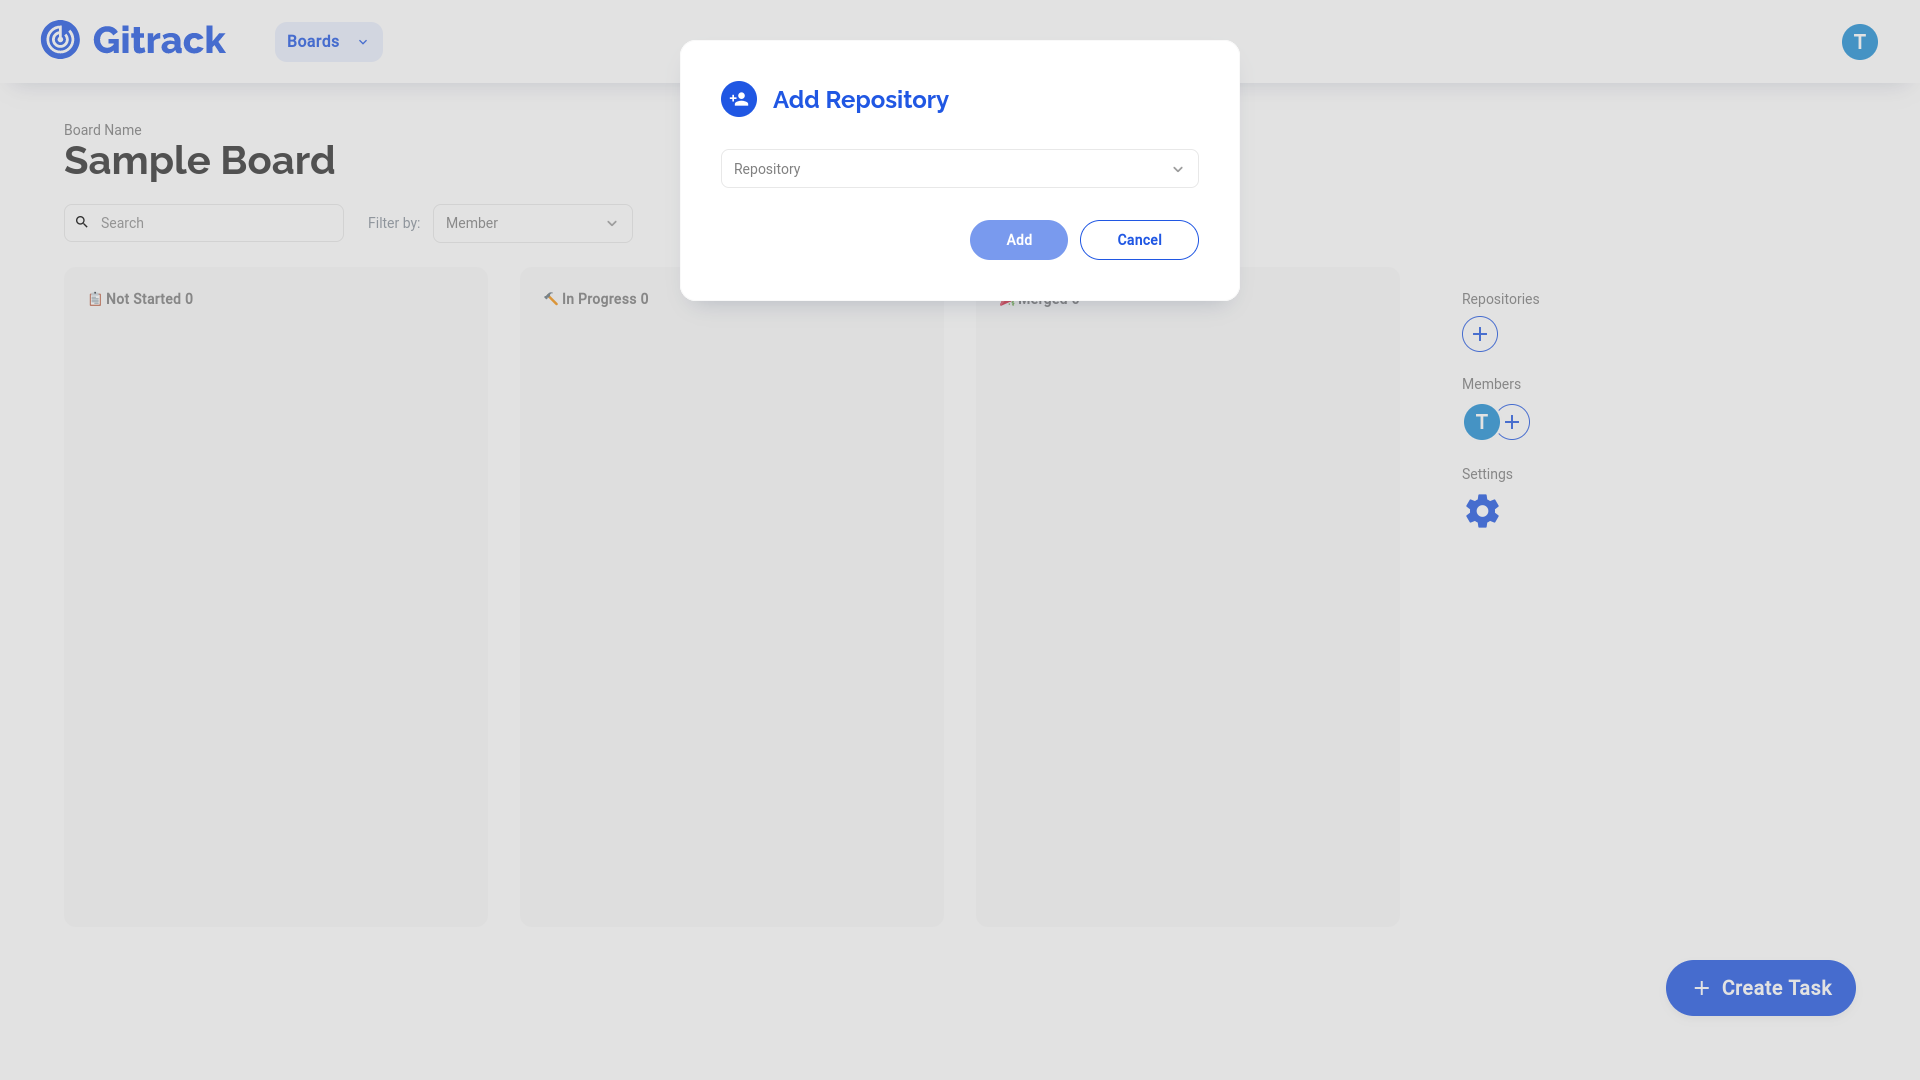
\includegraphics[width=1\textwidth]{add-repo}\par\vspace{0.5cm}
	\caption{Add Repository Modal}
	\label{fig:add-repo}
\end{figure}

\subsubsection{Description}
The \emph{Add Repository} screen shows a modal with a dropdown menu that lists
the repositories of the GitHub-authenticated user. This allows the user to add a
repository to the current board and enables linking branches in the said
repository to tasks.

\subsubsection{Frontend}
Add Repository is a modal that only gets displayed when the ``Add'' button under
``Repositories'' on the board is clicked and if the user has already connected
their Github account. It was implemented using a modal component with the same
UI elements such as the buttons, icon, and title as other modals of the same
size. The only difference is the title, the ``action'' of the primary button
which is ``Add'', and, importantly, the content of the modal itself which is a
dropdown menu which lists all the repositories in the user’s Github account.

\code{repos()}, which is one of the functions in \code{GithubService}, is
immediately called once Add Repository is opened. \code{repos()} is a GET
request to \code{/github/repos}. The server returns all the repositories
connected to the user’s account. The repositories’ full names are displayed
within the dropdown menu. Once a repository is chosen and the “Add” button is
clicked, the \code{connectRepo()} function is called which is from
\code{BoardService}. \code{connectRepo()} is a POST request to
\code{/board/\${boardId}/connect} that sends the \code{boardID,} the selected
repo’s \code{id}, \code{full\_name}, and \code{url}. This effectively assigns
the chosen repository to the board. \code{refreshBoardRepos()} is then called
and the modal is closed.

\subsubsection{Backend}
This is implemented using the \code{connectRepository()}, \code{getBoardById()},
and \code{getGithubToken()} functions. \code{connectRepository()} accepts four
parameters: 1. \code{id}: the repository ID from GitHub, 2. \code{name}: the
repository’s name, 3. \code{url}: the URL to the repository, and 4.
\code{boardId}: the id of the board to which the repository will be connected.
\code{connectRepository()} adds these values to the Repositories table.
\code{getBoardById()} returns an object containing a board’s information in the
\emph{Boards} table based on its unique id, which is accepted as a function
parameter id. \code{getGithubToken()} retrieves the user’s GitHub authentication
token from the database using their unique id, which is accepted as the function
parameter userId. If the user has not authenticated their GitHub account, they
will not have an authentication token in the database, and
\code{getGithubToken()} will throw and error message of
\code{NOT\_GITHUB\_AUTHENTICATED.}

The endpoint, \code{boards/connect}, receives a POST request with the board
\code{id} as a parameter. It also makes use of the user’s unique \code{id} to
check for the required permissions. The request body contains: \code{repo\_id},
the repository ID from GitHub; \code{full\_name}, the full name of the
repository from GitHub; and \code{url}, the URL to the repository. The endpoint
returns a JSON with keys \code{id}, \code{full\_name}, \code{board\_id}, and an
\code{error\_message}. First, the endpoint checks if any of the \code{ids},
\code{fullName}, or \code{url} are missing. If it is missing, the endpoint
returns a status code 400 with null values for the JSON keys and an
\code{error\_message} of \code{MISSING\_ID}, \code{MISSING\_FULL\_NAME}, and
\code{MISSING\_URL} respectively. The endpoint checks if the user is a developer
or a project manager with \code{getPermissions()}. The endpoint then retrieves a
\code{board} object and stores it in a variable \code{board}, whose properties
are the board information in the \emph{Boards} table, using the
\code{getBoardById()} function using the \code{id} request parameter as an
argument. If \code{getBoardById()} does not find a board with the specific
\code{id}, it returns \code{undefined} and \code{board} gets this value. In this
case, the endpoint returns status code 403 and null values for the JSON keys and
for security reasons, an error\_message of \code{NOT\_ENOUGH\_PERMISSIONS}. If
board is not \code{undefined}, the endpoint proceeds to retrieve the user’s
GitHub authentication token using \code{getGithubToken()} and stores it in a
variable \code{authToken}. If this fails, the endpoint returns a status code 403
with null values for the JSON keys and the \code{error\_message} thrown by
\code{getGithubToken()}. If it succeeds, the endpoint proceeds to connect the
repository to the board using \code{connectRepository()}, and creates a webhook
to the repository (see Section M). If \code{connectRepository()} fails, the
endpoint returns a status code 500 with null values for the JSON keys and the
\code{error\_message} thrown by \code{connectRepository()}. If it succeeds, it
returns a status code 200 with the JSON keys having the following values: repoId
for the \code{id} key, fullName for the \code{full\_name} key, the id request
parameter for the \code{board\_id} key, and a null value for the
\code{error\_message} key.

\subsection{Add Members}
\begin{figure}[H]
	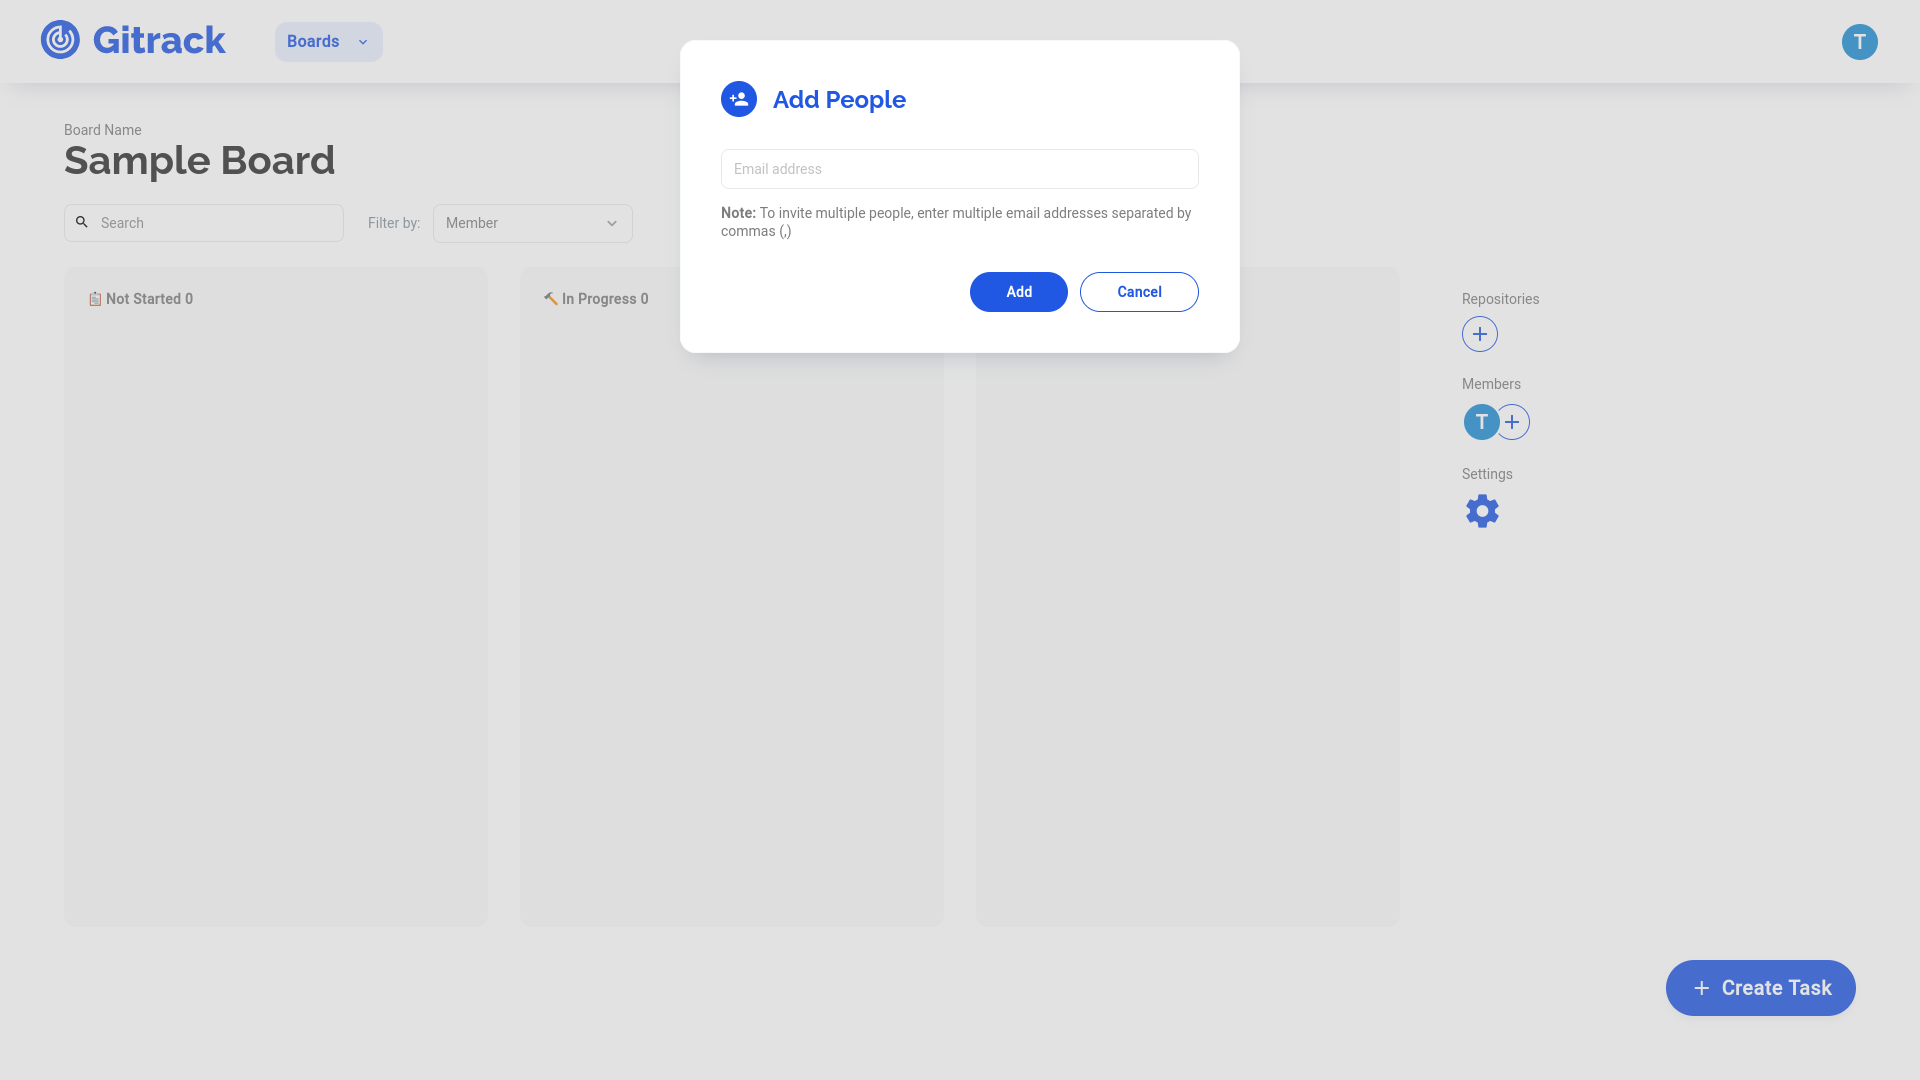
\includegraphics[width=1\textwidth]{add-member}\par\vspace{0.5cm}
	\caption{Add Members Modal}
	\label{fig:add-member}
\end{figure}
\subsubsection{Description}
The Add Members shows a modal with an input form that lets the user type-in an
email of other existing users for them to be added to the board.

\subsubsection{Frontend}
Add Members is a modal that only gets displayed when the “Add” button under
“Members” on the board is clicked. It uses the same modal component and UI as
the previous component, Add Repository. The only difference with Add Repository
is the title, the subtext under the input field that contains instructions on
how to add members, and the input field for the email addresses.

In order to add a member to the board, the user must enter the specific member’s
email address. As stated in the note underneath the input field, it is possible
to add multiple members by separating the email addresses with commas. Once the
“Add” button is clicked, the \code{onSubmit} function is called. This takes the
email/s entered and passes them as arguments for the \code{exists()} function
found in \code{UserService}. This is a GET request to \code{/user/exists}. If
the emails are connected to existing users, their ids are returned. The
\code{addDevelopers()} function from \code{BoardService} is then called.
\code{addDevelopers()} is a POST request to
\code{/board/\${boardId}/add-developer} that sends the \code{board\_id} and the
\code{developer\_ids} to be added as members to the corresponding board back to
the server. \code{refreshBoardMembers()} is then called and the modal is closed.

If one or more emails aren’t connected to any users, the \code{exists()}
function returns null. An error message is then displayed indicating “One or
more users do not exist.”

\subsubsection{Backend}
This was implemented through a function \code{addDevtoBoard()} which accepts the
parameters \code{boardId} and \code{devId}. It then checks if the User with
\code{id} specified in \code{devId} exists in the database. If the user does
exist, it is then added into the \emph{Memberships} table. Otherwise throws an
error \code{USER\_NOT\_FOUND}. If inserting into the \emph{Memberships} table
fails, \code{INSERT\_FAILED} error is then thrown.

For its endpoint,
\code{boards/:id(\textbackslash{}\textbackslash{}d+)/add-developer}, receives a
POST request which accepts an \code{id} from the request parameter, accepts
\code{userId} from the user, and accepts \code{developer\_ids} from the request
body. It also returns a JSON with the keys \code{board\_id}, \code{dev\_id},
\code{duplicate\_devs}, and \code{error\_message}. An empty array of developer
IDs is then declared. It checks if the \code{id} is undefined. If it is, then it
responds with status code 400, returns \code{null} value for the JSON keys, and
an \code{error\_message} of \code{MISSING\_ID}. After, it checks if the user has
permissions to do this function by trying the \code{getPermissions()} function.
If it fails, then it responds with a 403 status code, also returns \code{null}
for the JSON keys, and the thrown error from the \code{getPermission()} function
for the \code{error\_message}. And if the user has permissions, it then proceeds
to try and call \code{addDevtoBoard()} function. If the developers have
successfully been added, it then responds and returns \code{id} for
\code{board\_id}, string converted \code{devsToAdd} for \code{dev\_id}, filtered
\code{devIds} for the \code{duplicate\_devs}, and \code{null} for the
\code{error\_message}. If it fails to add the developers to the board, it
responds with a 500 status code, returns \code{null} for \code{board\_id},
\code{dev\_id}, and \code{duplicate\_devs} keys, and an \code{error\_message}
from the error thrown of \code{addDevToBoard()} function.


\subsection{Create Task}
\begin{figure}[H]
	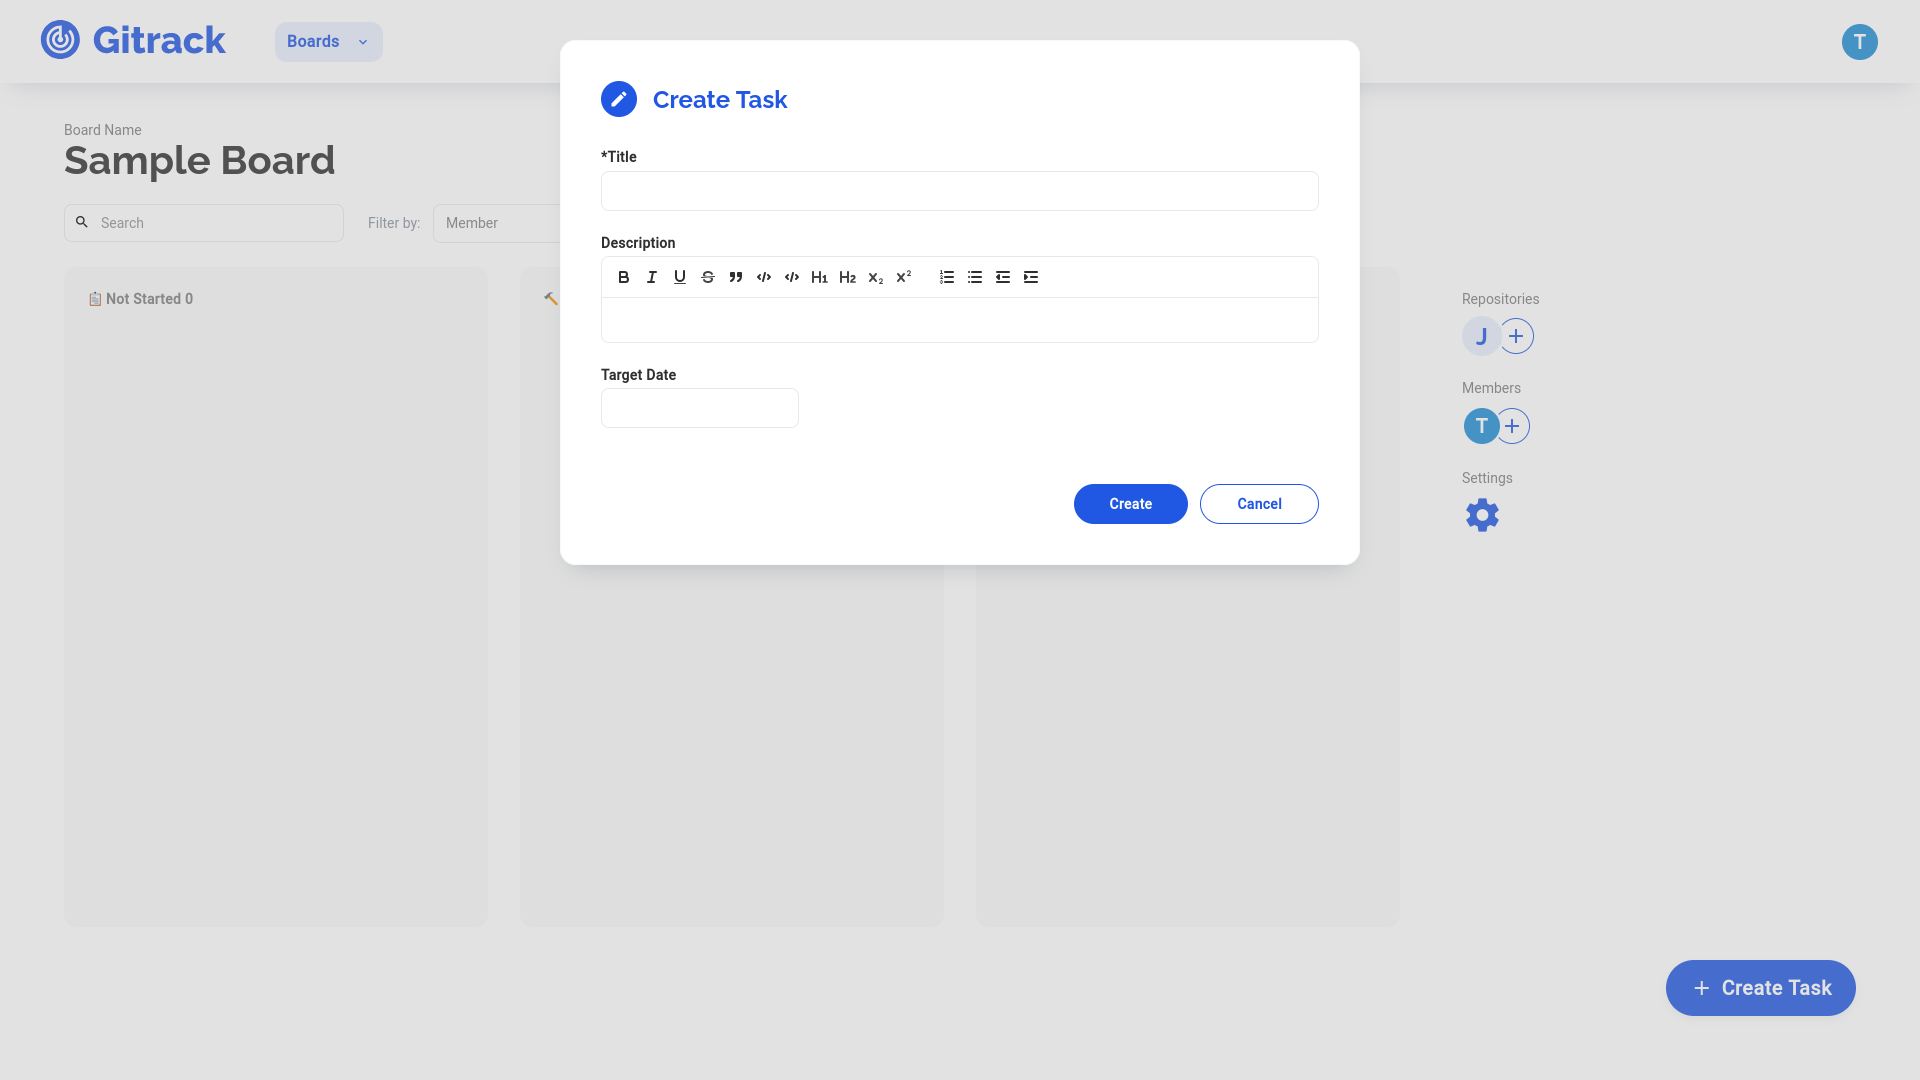
\includegraphics[width=1\textwidth]{create-task}\par\vspace{0.5cm}
	\caption{Create Task Modal}
	\label{fig:create-task}
\end{figure}

\begin{figure}[H]
	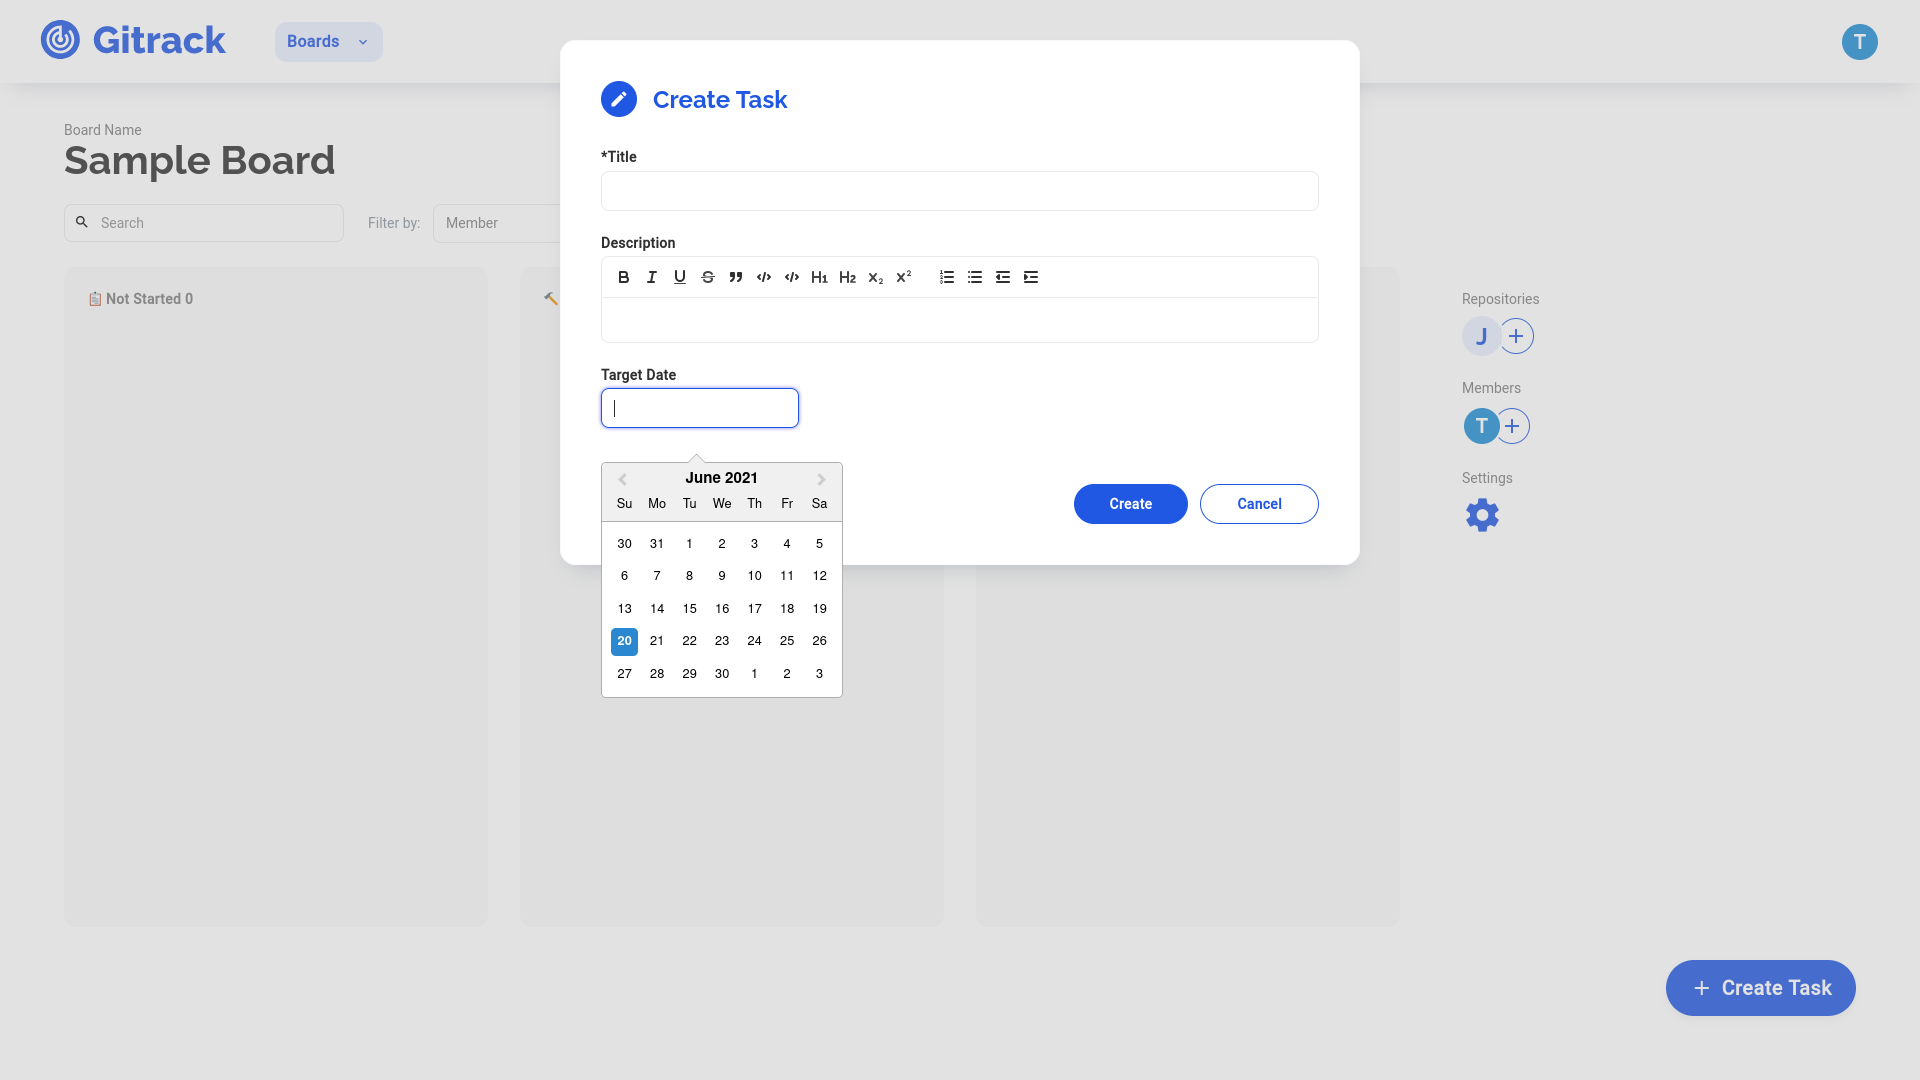
\includegraphics[width=1\textwidth]{create-task-date}\par\vspace{0.5cm}
	\caption{Create Task Modal with Target Date input clicked}
	\label{fig:create-task-date}
\end{figure}

\subsubsection{Description}
The Create Task component shows a modal that lets the user enter the
specifications of their task. The specification includes the title of the task,
description, and target date. Out of the three fields, only the title is
required to be able to successfully create a task.

\subsubsection{Frontend}
The three inputs in the Create Task component function very differently from one
another. The Title input is a very simple input that is only capable of plain
text. The Description input is a rich text editor that is capable of formatting
text. This allows the user to emphasize key words or phrases, add numbering or
even add bullet points. This was possible through the integration of an open
source WYSIWYG editor known as \emph{Quill}. Lastly, the Target Date input, when
clicked, displays a calendar that would set the date by selecting the desired
date on the calendar. This was implemented using an open source datepicker
component known as \emph{React Datepicker}. Once the user clicks the ‘Create’
button, an \emph{onSubmit()} function is triggered. It first checks whether the
Title input is filled, since it is the only one that is required to create a
task. If it isn’t, it would display an error message telling the user to fill in
the input. After that, the \code{create()} function from the \code{TaskService}
would then be called. The \code{create()} function is a POST request to
\code{/task} that sends the \code{board\_id}, \code{title}, \code{description},
and \code{target\_date} as its body. Once successful, it retrieves the updated
list of tasks in the board by calling the \code{refreshBoardTasks()} function
and would then proceed to close the modal.

\subsubsection{Backend}
This component is implemented through a function \code{addTask()} which accepts the
parameters \code{title}, \code{description}, \code{targetDate}, and \code{boardId}. It then tries to insert
into the \emph{Tasks} table in the database. If insert is successful, it returns the
last ID that was inserted. Otherwise, throws an error of \code{INSERT\_FAILED}.

For this component’s endpoint, it receives a POST request which accepts
\code{board\_Id}, \code{title}, \code{description}, and \code{target\_date} from
the request body, and \code{userId} from the user. It also returns a JSON with
\code{id}, \code{column\_id}, \code{board\_id}, \code{title},
\code{description}, \code{target\_date}, and \code{error\_message} keys. It then
checks if \code{boardId}, \code{title}, \code{description}, and
\code{targetDate} are undefined. If one those are undefined, it responds with
400 status code, returns an \code{error\_message} of \code{MISSING\_BOARD\_ID},
\code{MISSING\_TITLE}, \code{MISSING\_DESCRIPTION}, and
\code{MISSING\_TARGET\_DATE} respectively, and \code{null} values for JSON keys.
After, it checks if the user has permissions to do this function by trying the
\code{getPermissions()} function. If it fails, then it responds with a 403
status code, also returns \code{null} for the keys, and an error thrown from the
\code{getPermission()} function for the \code{error\_message}. And if the user
has permissions, it then proceeds to try and call \code{addTask()} function. If
it is successful, it then responds and returns taskId for \code{id}, \code{0}
for \code{column\_id}, \code{boardId} for \code{board\_id}, \code{title},
\code{description}, \code{targetDate} for \code{target\_date} key, and
\code{null} for the \code{error\_message}. If it fails to add the developers to
the board, it responds with a 500 status code, returns \code{null} for the JSON keys,
and an \code{error\_message} from the error thrown by the \code{addTask()} function.

\subsection{Task Card}
\begin{figure}[H]
	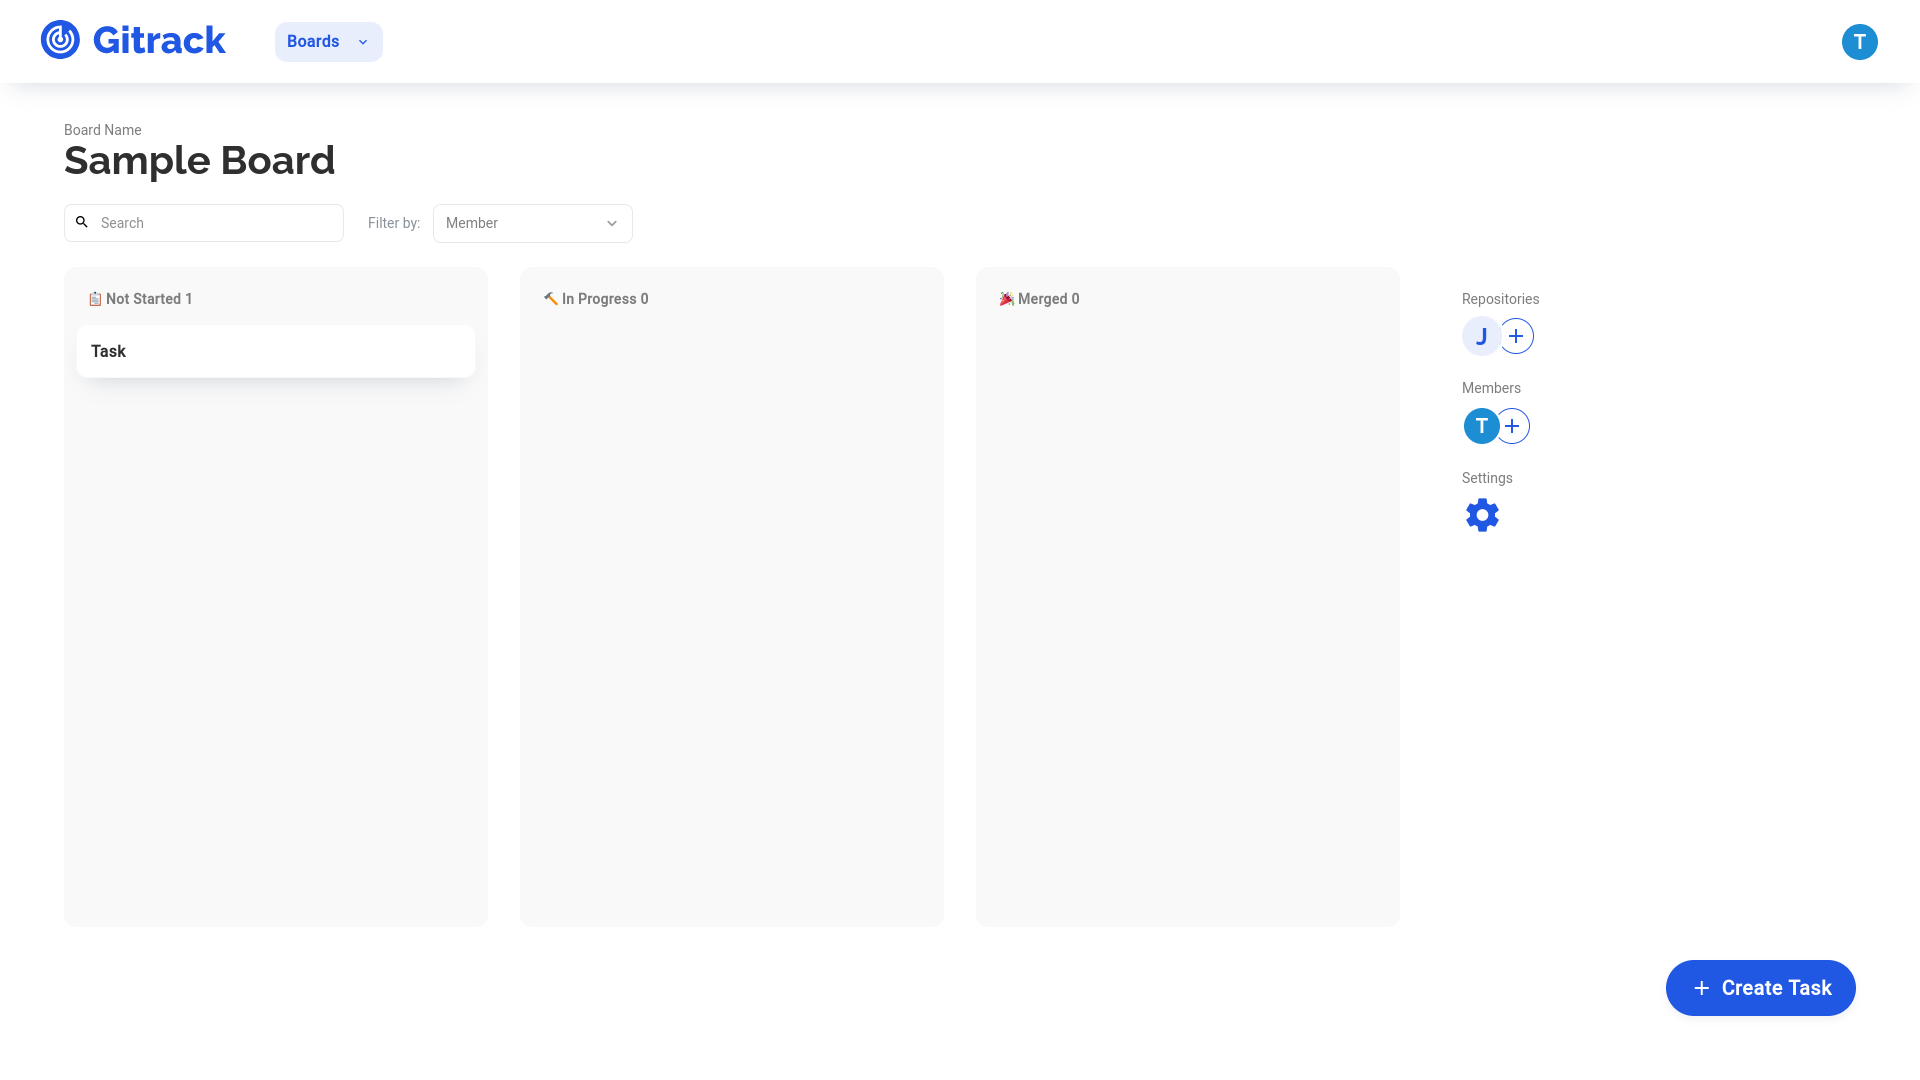
\includegraphics[width=1\textwidth]{task-not-started}\par\vspace{0.5cm}
	\caption{Task Card in Not Started Column}
	\label{fig:task-not-started}
\end{figure}

\begin{figure}[H]
	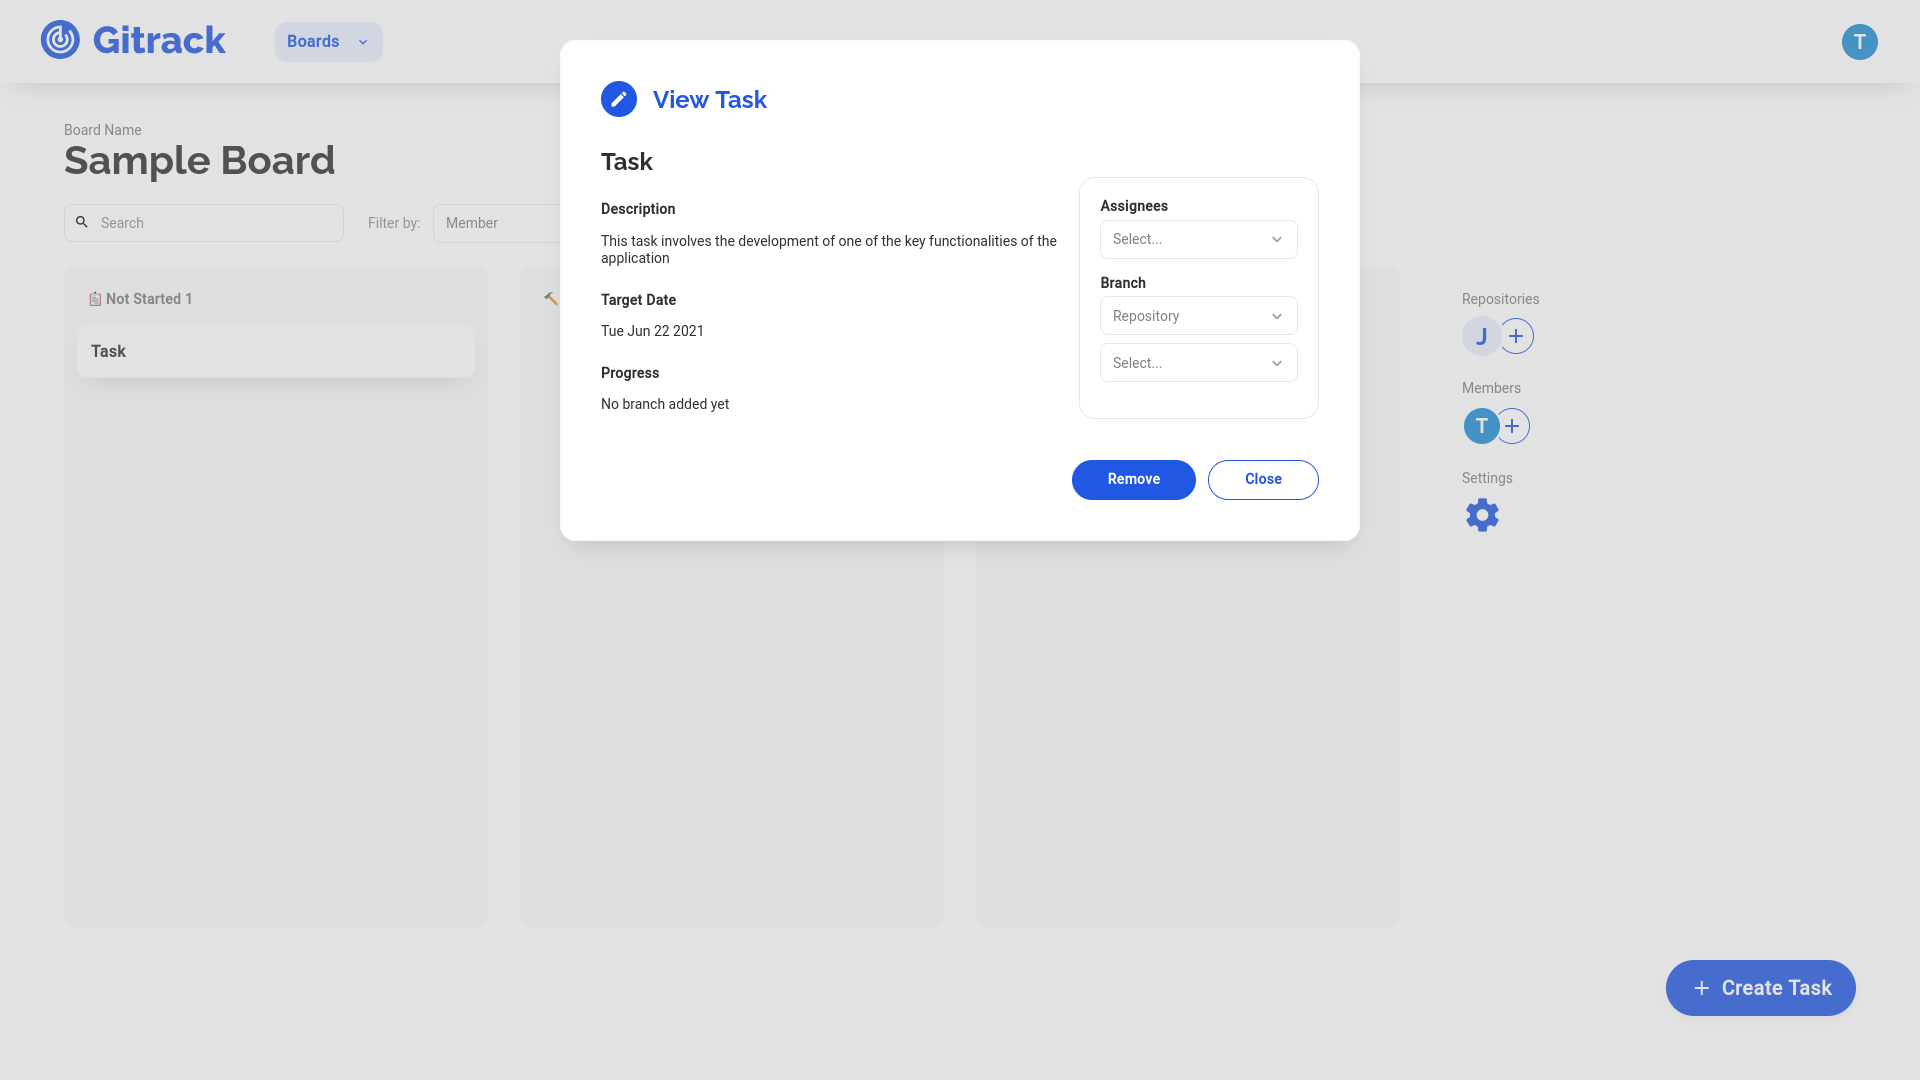
\includegraphics[width=1\textwidth]{view-task}\par\vspace{0.5cm}
	\caption{View Task Modal}
	\label{fig:task-in-progress}
\end{figure}

\begin{figure}[H]
	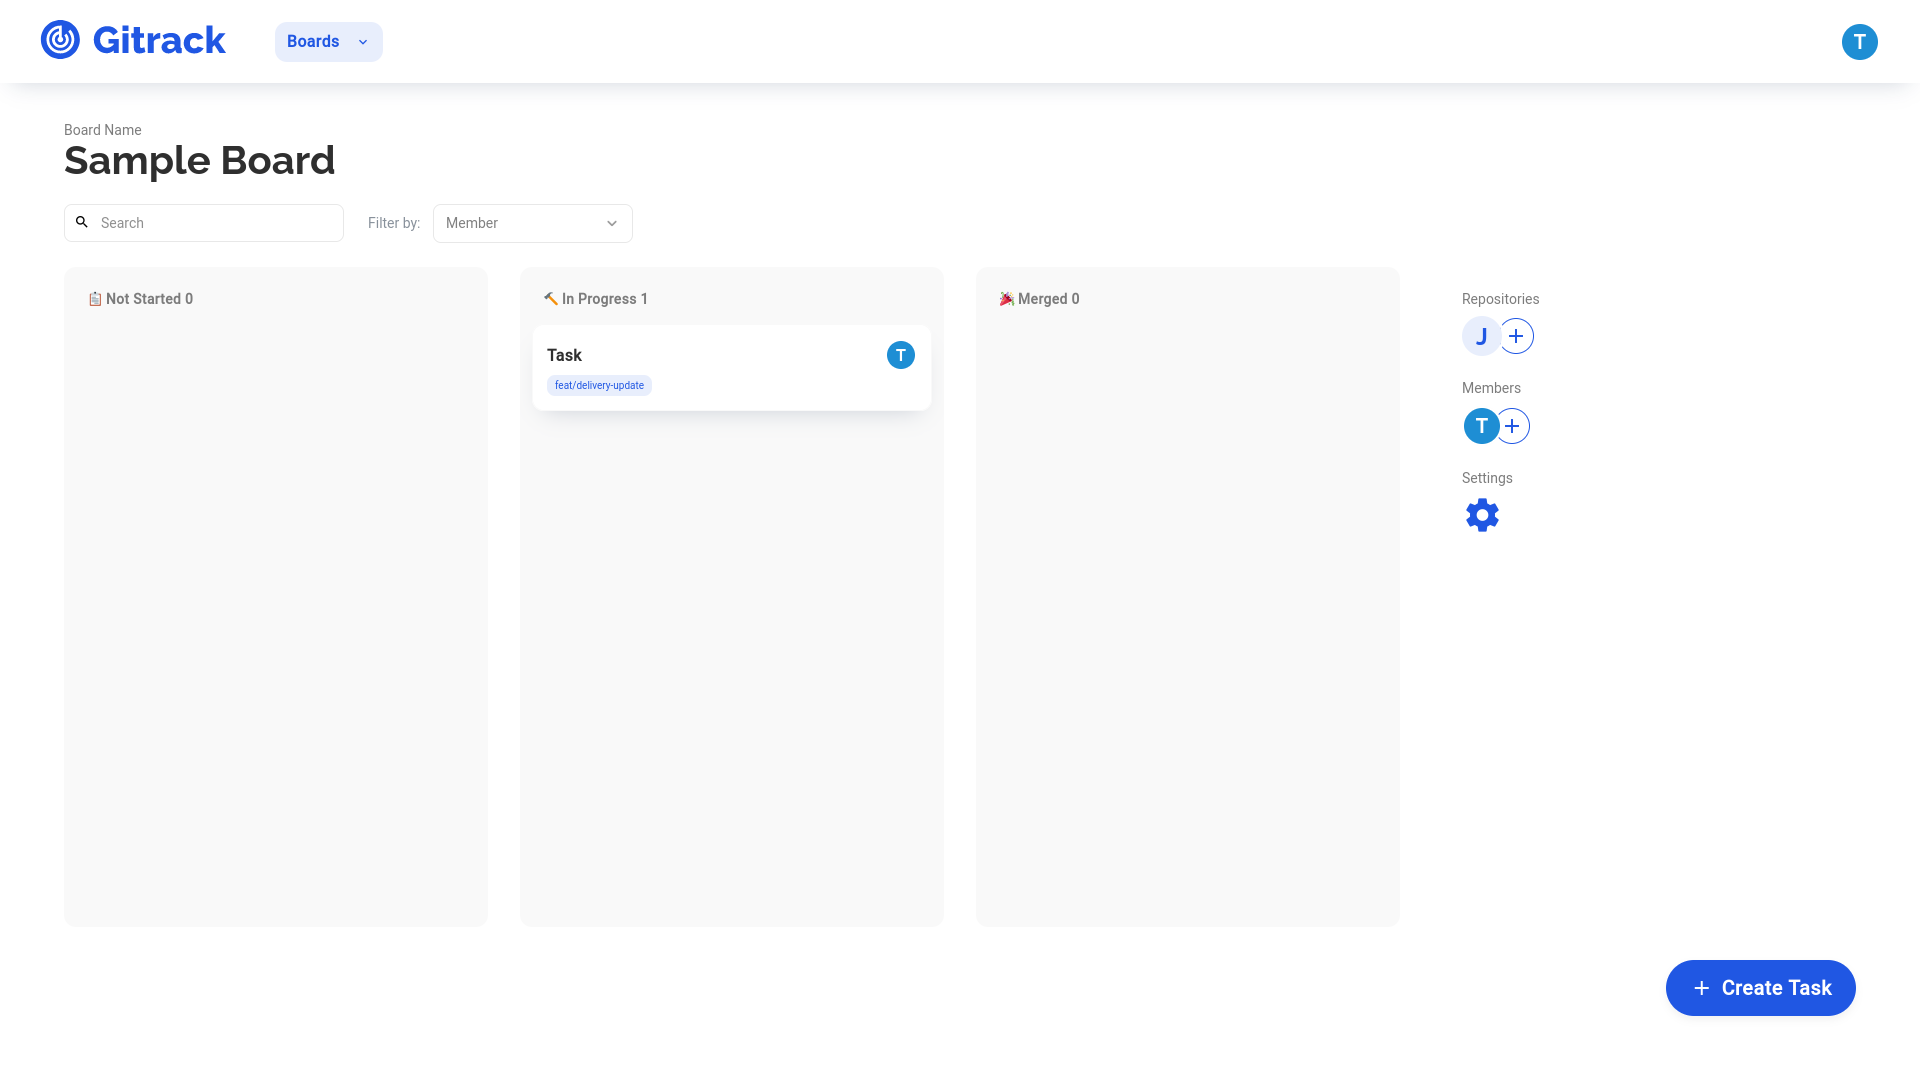
\includegraphics[width=1\textwidth]{task-in-progress}\par\vspace{0.5cm}
	\caption{Task Card in In Progress Column}
	\label{fig:task-in-progress}
\end{figure}
\subsubsection{Description}
The Task Card component represents a task in the project. When the task is first
created, the task is placed in the Not Started column and the Task Card would
only display the task’s title, but once the task’s information is updated, such
as the assignees and the linked branch, it would be updated to display those as
well. Once the task is linked to a branch, it would automatically be transferred
to the In Progress column, and once the branch linked to it is merged, it will
then be transferred to the Merged column. In order to update the task’s
information, the user would have to click the Task Card to open the View Task
modal.

The View Task modal allows the user to view more information about the task, as
well as modify information that would most likely be updated throughout the
task’s lifetime such as its assignees and the branch it is linked to. It also
gives the user the ability to delete the task when the need arises.

\subsubsection{Frontend}
\paragraph{Task Card}
The Task Card, from the name itself, uses a simple Card component with custom
design elements. It displays the essential information of each task: the task’s
title, the icon of the member assigned, indicators for the deadline, and the
branch linked to the card. If the cursor is hovered above the task card, the
card’s color changes to a light blue from the normal white.

Everytime the card is rendered, the state of the task’s progress relative to the
deadline is checked. Using the current date and the target date of the task, it
is determined whether the task has gone beyond the deadline without being
completed or merged. If the current date is beyond the task date, a warning icon
is then displayed next to the title of the card and the card’s border color is
changed to red.

\paragraph{View Task}
The View Task modal is opened once the Task Card is clicked. This modal is
larger in size and shares design elements with other modals. At the bottom right
of the modal is the Remove and Cancel buttons. The Remove button in blue opens
the Remove Task Modal while the Cancel button closes the View Task Modal.
Clicking outside of the modal also effectively closes the modal.

Much like in Task Card, once the modal is opened it immediately checks the
task’s progress relative to the deadline. If the current date is past the task
deadline, a warning icon is displayed next to the Target Date.

\paragraph{Remove Task}
The Remove Task modal is opened once the Remove button on View Task modal is
clicked. It shares the same UI elements as other modals of the same size except
the content simply asks “Are you sure you want to remove this task?”

Once the Yes button is clicked to confirm the removal, the \code{remove()}
function is called from \code{TaskService}. This is a DELETE request to
\code{/task/\${taskId}} that sends the taskId as the body. If the delete is
successful, \code{refreshBoardTasks()} is called and the modal is closed.

\paragraph{Setting Assignees}
To the right of the View Task modal, a card houses the dropdown menus for the
list of members that could be assigned to the task. Once the View Task modal is
opened, it immediately checks if there are members assigned to the task already.
From the dropdown menu, the user can simply click on the name of the member they
would like to assign to the task.

Once the modal is closed, if there are developers selected and no members have
been assigned to the task before, the \code{assign()} function is called from
\code{TaskService}. This is a POST request to
\code{/task/\${taskId}/assign-task} which sends the \code{task\_id},
\code{board\_id}, and \code{assignee\_ids}. If there were already assigned
members beforehand and there is another developer selected, the
\code{updateAssignees()} function is called from \code{TaskService} which is a
PUT request to \code{/task/\${taskId}/assign-task} that sends the same data. If
the request response is successful, the function \code{refreshBoardTasks()} is
called and the modal is closed.

\paragraph{Connect Branch}
Right under the assignees dropdown menu are the dropdown menus for the
repository and branch that could be assigned to the task. If there is no
repository assigned to the task yet, the repositories linked to the board are
all listed. Once the user selects a repository, the specific branches in that
repository are then displayed in the dropdown menu for branches. Once a branch
is selected or if there already was a selected branch before and a new branch is
selected, the \code{connect()} function from \code{TaskService} is called. This
is a PATCH request that sends the \code{repo\_id} of the selected branch, the
name of the selected branch, and the \code{taskId}. This updates the branch
connected to the specific task.

\subsubsection{Backend}
\paragraph{View Task}
From the \code{/board/:id(\textbackslash{}\textbackslash{}d+)/tasks} endpoint
used in the Main Dashboard (see Section F), an array of objects containing all
the task information in the board is obtained and the values of the properties
of these objects are displayed in the frontend.

\paragraph{Remove Task}
This is implemented through a function \code{removeTask()} which accepts the
parameter \code{id}. Through this \code{id}, the \code{id} in the \emph{Tasks}
table it corresponds to is deleted. If the result.changes is zero (0), it means
such a task does not exist, throwing an error of \code{TASK\_NOT\_FOUND}.
Otherwise, the \code{id} is returned. If unsuccessful, it throws an error. The
\code{removeTask()} is then called in the
\code{tasks/:id(\textbackslash{}\textbackslash{}d+)} endpoint. This endpoint
receives a DELETE request which accepts \code{id} from request parameters, and
\code{userId} from the user. This also returns a JSON with keys \code{id},
\code{column\_id}, \code{board\_id}, \code{title}, \code{target\_date}, and
\code{error\_message}. It first checks if the task exists. If it exists, then
checks if the user has permissions through the \code{getPermissions()} function.
After, the \code{removeTask()} is then called. If successful, returns a JSON of
the task, and \code{null} value for \code{error\_message} key.

\paragraph{Set Assignees}
This is implemented through the function \code{setAssignees()} which accepts the
parameters \code{taskId}, and \code{assigneeIds}. It is then followed by a try
catch in which \code{assigneeIds} are individually inserted into the
\code{Assignees} table along with the \code{taskId}. If it fails, it is then
caught, and an error \code{INSERT\_FAILED} is thrown. This function is then
called in the \code{tasks/:id(\textbackslash{}\textbackslash{}d+)/assign-task}
endpoint. This endpoint receives a POST request which accepts \code{id} from
request parameters, \code{userId} from the user, and \code{board\_id,}
\code{assignee\_ids} from the request body. This also returns a JSON with keys
\code{board\_id}, \code{task\_id}, \code{assignee\_ids}, and
\code{error\_message}. It first checks if the user has permissions through
\code{getPermissions()} function. If the user has permission, then the
\code{setAssignees()} is then called. If successful, returns a JSON with
\code{boardId} value for \code{board\_id}, \code{id} value for \code{task\_id}
key, \code{assigneeIds} value for \code{assignee\_ids} key, and \code{null}
value for \code{error\_message} key.

\paragraph{Connect Branch}
This is implemented through function \code{connectBranch()} which accepts the
parameters \code{task\_id}, \code{branch}, and \code{repoId}. The row of the
\code{taskId} in the \emph{Tasks} table is then updated with the repository ID
(\code{repoId}) and branch (\code{branch}) it corresponds to. If unsuccessful,
an error message of \code{CONNECTION\_FAILED} is thrown. The
\code{connectBranch()} function is then called in the
\code{tasks/:id(\textbackslash{}\textbackslash{}d+)/connect} endpoint. This
endpoint receives a PATCH request which accepts \code{id} from request
parameters, \code{userId} from the user, and \code{repo\_id},
\code{branch\_name} from the request body. This also returns a JSON with keys
\code{name}, \code{repo\_id}, and \code{error\_message}. It first checks if the
\code{id}, \code{repoId}, and \code{branchName} are undefined. If at least one
is \code{undefined}, an error is thrown. Then, the \code{connnectBranch()} is
then called. If successful, returns a JSON with \code{branchName} value for name
\code{key}, \code{repoId} value for \code{repo\_id} key, and \code{null} value
for \code{error\_message} key.


\subsection{Task Card: View Commits}
\begin{figure}[H]
	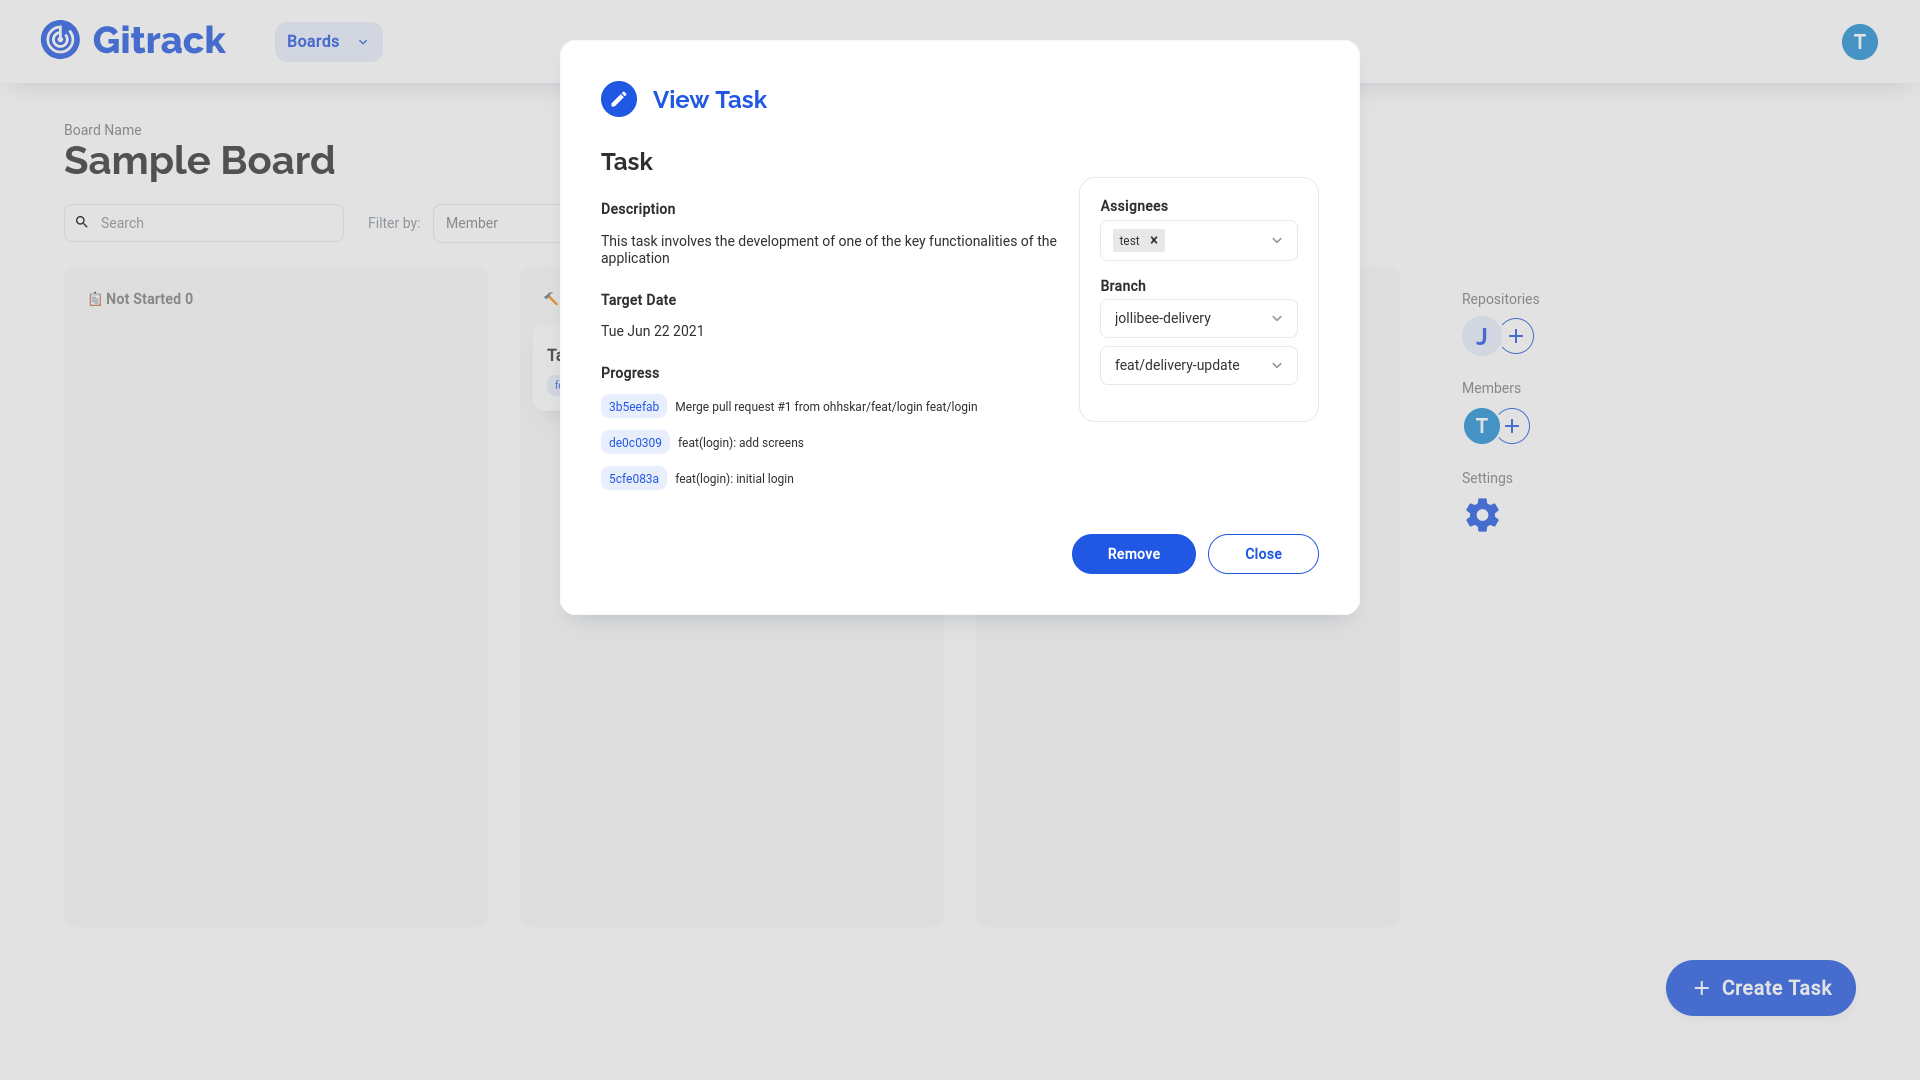
\includegraphics[width=1\textwidth]{view-task-commit}\par\vspace{0.5cm}
	\caption{View Task Modal with Commits}
	\label{fig:view-task-commit}
\end{figure}

\subsubsection{Description}
The View Commits component is only available to task cards whose tasks are
linked to a branch in GitHub. The task card can then display the three latest
commits to the branch linked to the task.

\subsubsection{Frontend}
Once the View Task Modal is opened and a branch has already been linked to the
task, or when the developer has just finished linking the task to a branch, the
component would then proceed to call the \code{commits()} function from \code{GithubService}.
The \code{commits()} function is a GET request to \code{/github/\${repoId}/commits} that
retrieves the list of commits given a \code{repo\_id} and \code{branch\_name.} This function
would also be called whenever the developer decides to link a different branch.
Once the server returns the list of commits, the component would then only
display the three latest commits from that branch.

\subsubsection{Backend}
This is implemented directly at its endpoint. It receives a GET request which
accepts \code{id} from the request parameter, and accepts \code{userId} from the
user. Three variables are declared with null values, namely \code{authToken},
\code{fullName}, and \code{rep}. It first checks if the \code{id} is
\code{undefined}, and if it is, then responds with 400 status code, returns
\code{null} value for \code{id} and \code{title}, and an \code{error\_message}
of \code{MISSING\_REPO\_ID}. If \code{id} is defined, it then proceeds to try
and call \code{getGithubToken()} function to get an authentication token for the
user. If unsuccessful, it responds with 403 status code, returns \code{null}
value for the branches, and an \code{error\_message} from the function. If
successful, it then tries and calls \code{getRepository()} function. If it
fails, it responds with 400 status code, returns \code{null} value for the
branches, and an \code{error\_message} from the thrown error of the
\code{getRepository()} function. Otherwise, the returned string of the
\code{getRepository()} function which is stored in the \code{fullName} variable
is split with ‘/’ and is assigned to the \code{rep} variable. After, POST GitHub
endpoint \code{/repos/{owner}/{repo}/commits} is called to get the commits, and
then stored in \code{data}. If successful, \code{data} is then mapped to get the
required elements from the list of commits which are the hashes, url, and commit
message. It then returns a JSON of the mapped commits, and \code{null} value of
\code{error\_message}. If the request failed, the error status is checked. If
error status is 401, \code{removeGithubToken()} is called, then it responds with
403 status code, returns \code{null} value of \code{repos}, and an
\code{error\_message} of \code{NOT\_GITHUB\_AUTHENTICATED}. If not 401, then it
responds with 403 status code, returns null value of repos and the error from
the recent try catch.

\subsection{Automatic Movement of Cards}
\subsubsection{Description}
A key differentiator of GiTrack over other project management tools is the
ability to automatically move cards depending on the git status of the
accompanying branch. If a task has a connected branch, this task will be
automatically moved to the next column: “In Progress”. Once a feature branch has
been completed and merged to the main branch, the task will be automatically
moved to the final column: “Completed”.

\subsubsection{Backend}
There are two ways the backend moves the cards. The first method is done when a
card is moved from “To Do” to “In Progress”. The movement of a card of this type
is done when a branch is connected to the task. As such, this functionality
piggybacks on the \code{task/{id}/connect} endpoint. When this endpoint is
called, the function \code{connectBranch()} is called. This function is
described in full on Section K. One specific change this function has is
updating the \code{column\_id} column on a task. It sets this \code{column\_id}
to 1 which indicates that this task is now on the “In Progress” column.

The second method handles the instance where a card moves from “In Progress” to
“Completed”. This is done by detecting the moment a branch is merged and
checking if that branch is connected to a task. To accomplish this a webhook is
attached to a repository once it has been connected. This is done by the
\code{board/{id}/connect} endpoint. The full functionality of this endpoint is
described in Section H. A part of the functionality of this endpoint is calling
the POST GitHub endpoint \code{/repos/{owner}/{repo}/hooks} with a config that
indicates that the application is interested in receiving all events that
correspond to pull requests. GitHub sends this information to the application by
sending a POST request to \code{/github/payload}. This endpoint checks the type
of payload that GitHub has sent. If it is a \code{pull\_request} payload, the
endpoint checks if that specific event is closing and merging a pull request. If
so, it calls the function \code{moveTaskByBranchAndRepo()} which has
\code{branchName}, \code{repoId}, and \code{columnId} as arguments.
\code{branchName} specifies the full branch name, \code{repoId} is the ID of the
repository where the pull request was merged, and \code{columnId} is the column
where that task is to be moved. In this case, \code{columnId} was set to 2,
which means that the task should be moved to the “Completed” column.

\end{document}
